\documentclass[a4paper, notitlepage, 11pt]{article}
\usepackage{geometry}
\fontfamily{times}
\geometry{verbose,tmargin=30mm,bmargin=25mm,lmargin=25mm,rmargin=25mm}
% end configs
\usepackage{setspace,relsize}               
\usepackage{moreverb}                        
\usepackage{url}
\usepackage{hyperref}
\hypersetup{colorlinks=true,citecolor=blue}
\usepackage{subfigure}
\usepackage{enumitem}
\usepackage{amsmath}
\usepackage{mathtools} 
\usepackage{amsthm}
\usepackage{amsmath}
\usepackage{amssymb}
\usepackage{indentfirst}
\usepackage{todonotes}
\usepackage[authoryear,round]{natbib}
\bibliographystyle{apalike}
\usepackage[pdftex]{lscape}
\usepackage[utf8]{inputenc}
\usepackage{multirow}
% \usepackage{multicolumn}

% Title Page
\title{\vspace{-9ex}\centering \bf On properties of the normalized power prior}
\author{
% Luiz Max de Carvalho\\
% Program for Scientific Computing (PROCC), Oswaldo Cruz Foundation. \\
}
\DeclareMathOperator*{\argmin}{arg\,min}
\DeclareMathOperator*{\argmax}{arg\,max}
\newtheorem{theorem}{Theorem}[]
\newtheorem{lemma}{Lemma}[]
\newtheorem{proposition}{Proposition}[]
\newtheorem{remark}{Remark}[]
\setcounter{theorem}{0} % assign desired value to theorem counter

% \setenumerate[1]{align=left,label=\arabic*}
% \setenumerate[2]{before=\stepcounter{enumi},label*=.\arabic*,leftmargin=1.2em,align=left}


\begin{document}
\maketitle

% \begin{abstract}
% 
% Key-words: ;; ; ; . 
% \end{abstract}

\section{Background}

\begin{itemize}
 \item Power priors are cool. [bunch of citations for propriety of GLM, Cox model, exponential family, etc];
 \item In this paper we explore the situation where the initial prior $\pi$ is proper;
 \item We also explore ways of approximating the normalising constant $c(a_0)$ for models where it cannot be written in closed-form. 
\end{itemize}

\textbf{Definition}
The data $D_0 = \{ d_{01}, \ldots, d_{0N_0} \} \in \mathcal{X} \subseteq \mathbb{R}^p$ are assumed independent and identically distributed  and the parameter $\theta \in \Theta \subseteq \mathbb{R}^q$ and $a_0 \geq 0$.
\begin{equation}
\label{eq:power_prior}
 p(\theta \mid D_0, a_0) \propto L(D_0 \mid \theta)^{a_0}\pi(\theta).
\end{equation}

[DEFINE UNORMALISED POWER PRIOR]

[DEFINE NORMALISED POWER PRIOR]

[CITE DUAN] 

\begin{equation}
 \label{eq:joint_a0}
 p(\theta, a_0 \mid D_0, D, \delta) \propto \frac{L(D_0| \theta)^{a_0} \pi(\theta) L(D | \theta) \pi_A(a_0)}{c(a_0)} 
\end{equation}

which leads to 
\begin{align}
 \nonumber
   p(a_0 \mid D_0, D, \delta)  &= \int_{\Theta}  p(\theta, a_0 \mid D_0, D, \delta) \, d\theta,\\
  \label{eq:marginal_posterior_a0}
  & \propto \frac{\pi_A(a_0)}{c(a_0)} \int_{\Theta}  L(D_0| \theta)^{a_0} \pi(\theta) L(D | \theta) \, d\theta
\end{align}
when the new data are an exact copy of the historical data, we have
$$  p(a_0 \mid D_0, D, \delta) \propto \frac{c(a_0 + 1)}{c(a_0)} \pi_A(a_0 \mid \delta) $$

\section{Theory}

We want to show under which conditions
\[\int_{\Theta} L( D_0 \mid \theta)^{a_0}\pi(\theta) \, d\theta <\infty.\]
\begin{theorem}
\label{thm:integrability}
 Assume $\int_{\mathcal{X}} L( x \mid \theta)dx < \infty$.
 Denote $f_{a_0}(D_0;\theta) : = L( D_0 \mid \theta)^{a_0}\pi(\theta)$.
 Then for $a_0 > 0$, $\int_{\Theta} f_{a_0}(D_0;\theta) \, d\theta <\infty$.
\end{theorem}
\begin{proof}
First, note that for $0 < a_0 \leq 1$, the function $g(x) = x^{a_0}$ is concave.
Then, by Jensen's inequality and the finiteness of $L( D_0 \mid \theta)$ for all of its arguments we have
\[ \int_{\Theta} f_{a_0}(D_0; \theta) \, \, d\theta \leq \left[ \int_{\Theta} L(D_0  \mid \theta)\pi(\theta) \, \, d\theta \right]^{a_0} < \infty. \]
Rewrite $f_{a_0}(D_0; \theta) = L(D_0 \mid \theta)^{a_0 -1} L(D_0 \mid \theta)\pi(\theta)$.
If $1 \leq a_0 \leq 2$, we have the Jensen's inequality case above, since we know that $L(D_0 \mid \theta)\pi(\theta)$ is normalisable.
Similarly, if $2 \leq a_0 \leq 3$, we can write 
\[  f_{a_0}(D_0; \theta) = L(D_0 \mid \theta)^{a_0-p} L(D_0 \mid \theta)^p\pi(\theta), \]
with $1 \leq p \leq 2$, again falling into the same case, since we know that $L(D_0 \mid \theta)^{p}\pi(\theta)$ is normalisable.
We can then show that for any $n \geq 1 \in \mathbb{N}$, $\int_{\Theta}f_{a_0}( D_0 ; \theta)\, d\theta < \infty$ for  $n-1 \leq a_0 \leq n$.
The base case for $1 \leq n \leq 3$ is established.
Now suppose the hypothesis holds for $n \geq 3$.
For $ n \leq  a_0 \leq n + 1$ and $n-1 \leq p_n \leq n$:
\begin{align*}
 \int_{\Theta} L(D_0 \mid \theta)^{a_0-p_n} L(D_0 \mid \theta)^{p_n}\pi(\theta)\, d\theta < \infty, \\
\end{align*}
because $0 \leq a_0 - p_n \leq 1$ and $L(D_0 \mid \theta)^{p_n}\pi(\theta)$ is proper by hypothesis, establishing the case for $n + 1$.
\end{proof}
\begin{remark}
 The power prior on multiple (independent) historical data sets is also a proper density.
\end{remark}
\begin{proof}
 Recall that the power prior on multiple historical data sets is of the form~\citep[Eq. 2.9]{Ibrahim2015}:
 \[ \pi(\theta \mid \boldsymbol D, \boldsymbol a_0) \propto \prod_{k=1}^K L(\theta \mid D_k)^{a_{0k}} \pi_0(\theta). \]
Assume, without loss of generality, that $L(\theta \mid  D_k)^{a_{0k}} > 1$ for all $\theta$ and let $m := \max(\boldsymbol a_0)$ with $\boldsymbol a_0 := \{ a_{01}, a_{02}, \ldots, a_{0K}\}$.
Then $\pi(\theta \mid \boldsymbol D, a_0)$ is bounded above by 
\[  g(\theta) :=  \prod_{k=1}^K L(\theta \mid D_k)^{m} \pi_0(\theta) =  \left[ \prod_{k=1}^K L(\theta \mid D_k) \right]^m  \pi_0(\theta) = L(\theta \mid \boldsymbol D)^m \pi_0(\theta), \]
which is normalisable following Theorem~\ref{thm:integrability}.
To relax the assumption made in the beginning, notice that this construction also bounds the case $ 0 \leq  L(\theta \mid  D_k)^{a_{0k}} \leq 1$ (for some $k$) above.
\end{proof}

\subsection{Properties of the normalising constant $c(a_0)$}
\label{sec:properties}

\begin{lemma}
\label{lm:convex_norm_constant}
Assume $L(D_0 \mid \theta)$ is continuous with respect to $\theta$.
Then the normalising constant is a strictly convex function of $a_0$.
\end{lemma}
\begin{proof}
Define the normalising constant as a function $c : [0, \infty) \to (0, \infty)$,
\begin{equation}
 \label{eq:normconst}
 c(a_0) := \int_{\Theta} L(D_0 \mid \theta)^{a_0} \pi(\theta)\, d\theta,
\end{equation}
which is positive and continuous on its domain.
The first and second derivatives are
\begin{align}
\label{eq:derivative_ca0}
c^\prime(a_0) &= \int_{\Theta} L(D_0 \mid \theta)^{a_0} \pi(\theta) \log L(D_0 \mid \theta) \, d\theta, \\
c^{\prime\prime}(a_0) &= \int_{\Theta} L(D_0 \mid \theta)^{a_0} \pi(\theta) [\log L(D_0 \mid \theta)]^2 \, d\theta,
\end{align}
and the integrals always exist (see Proposition~\ref{prop:c_is_Cinfinity} in Appendix~\ref{sec:further_proofs}).
Differentiation under the integral sign is justified because both $L(D_0 \mid \theta)^{a_0} \pi(\theta)$ and $L(D_0 \mid \theta)^{a_0} \pi(\theta) \log L(D_0 \mid \theta)$ are continuous with respect to $\theta$.
From this we conclude that $c$ is (strictly) convex and $c^\prime$ is monotonic, because $c^{\prime\prime}$ is always positive.
\end{proof}
For the goals of this paper, it would be useful to know more about the shape of $c(a_0)$, more specifically if and when its derivatives change signs.
% Let us first study an upper bound for $c^\prime(a_0)$.
% By a straight-forward application of the Cauchy-Schwarz inequality, we also know that $c^{\prime\prime}(a_0) \geq c^\prime(a_0)$.
% Now, to derive a lower bound on $c^\prime(a_0)$, consider the inequality $ 1- 1/x \leq \log(x)$, $x >0$, which suggests
% \begin{equation*}
%  \label{eq:c_a0_deriv_lb}
%  c^\prime(a_0) \geq c(a_0) - \int_{\Theta} L(D_0 \mid \theta)^{a_0-1} \pi(\theta) \, d\theta.
% \end{equation*}
For computational reasons, one is usually interested in $l(a_0) := \log(c(a_0)) $ instead of $c(a_0)$ and hence it is also useful to study the derivative of the log-normalising constant, $l^\prime(a_0) = c^\prime(a_0)/c(a_0)$.
A key observation is that $l^\prime(a_0)$ changes signs at the same point as $c^\prime(a_0)$ does, a feature we can exploit when designing algorithms for approximating $l(a_0)$ (see Section~\ref{sec:efficient_computation_ca0}).

\begin{remark}
 \label{rmk:discrete_decreasing}
 When $L(D \mid \theta)$ is a discrete likelihood, $c(a_0)$ is  decreasing in $a_0$.
\end{remark}
\begin{proof}
 The proof is immediate from Lemma~\ref{lm:convex_norm_constant} and the fact that for a non-degenerate discrete likelihood the function $\log(L(D\mid\theta))$ is negative and hence so is its expectation under the power prior.
\end{proof}

\subsubsection{Exponential family}
\label{sec:expo_family}

Suppose $L(D_0 \mid \theta)$ is in the exponential family:
\begin{equation}
 L(D_0 \mid \theta) = \boldsymbol h(D_0) \exp \left( \eta(\theta)^T \left(\sum_{i=1}^{N_0} T(d_{0i}) \right) - N_0 A(\theta) \right),
\end{equation}
where $\boldsymbol h(D_0) = \prod_{i = 1}^{N_0} h(d_{0i})$.
Thus we have
\begin{align}
 c(a_0) &=  \int_{\boldsymbol\Theta} \left[ \boldsymbol h(D_0) \exp \left( \eta(\theta)^T \left(\sum_{i=1}^{N_0} T(d_{0i}) \right) - N_0 A(\theta) \right) \right]^{a_0}\pi(\theta) \, d\theta, \\
  \label{eq:expo_family_const}
 &= \boldsymbol h(D_0)^{a_0}\int_{\boldsymbol\Theta} \exp \left( \eta(\theta)^T \left(a_0 \sum_{i=1}^{N_0} T(d_{0i}) \right) \right) \exp\left(- a_0N_0 A(\theta) \right) \pi(\theta) \, d\theta.
\end{align}
The derivative evaluates to 
\begin{equation}
\label{eq:expo_family_deriv_general}
 c^\prime(a_0) = \log(\boldsymbol h(D_0)) + \int_{\boldsymbol\Theta} \eta(\theta)^T \left(a_0 \sum_{i=1}^{N_0} T(d_{0i}) \right) f_{a_0}(D_0; \theta) \, d\theta -  a_0N_0\int_{\boldsymbol\Theta} f_{a_0}(D_0; \theta)  A(\theta) \, d\theta,
\end{equation}
where $f_{a_0}(D_0; \theta) := L(D_0 \mid \theta)^{a_0}\pi(\theta)$.

If we choose $\pi(\theta)$ to be conjugate to $L(D_0 \mid \theta)$~\citep{Diaconis1979}, i.e.
\begin{equation*}
 \label{eq:conj_exp_family}
 \pi(\theta \mid \tau, n_0) = H(\tau, n_0) \exp\{ \tau^T\eta(\theta) - n_0A(\theta) \},
\end{equation*}
we have 
\begin{align}
 \label{eq:expo_family_const_conj}
%  c(a_0) &= \boldsymbol h(D_0)^{a_0} H(\tau, n_0) \int_{\boldsymbol\Theta} \exp \left( \eta(\theta)^T \left(a_0 \sum_{i=1}^{N_0} T(d_{0i}) \right) -a_0N_0 A(\theta) \right) \exp\{  \eta(\theta)  \tau^T - n_0A(\theta) \} \, d\theta,\\
 c(a_0) &= \boldsymbol h(D_0)^{a_0} H(\tau, n_0) \int_{\boldsymbol\Theta}  \exp \left[ \eta(\theta)^T \left( \tau + a_0\sum_{i=1}^{N_0} T(d_{0i}) \right) -(n_0  + a_0N_0) A(\theta) \right] \, d\theta, \\
 &= \frac{\boldsymbol h(D_0)^{a_0} H(\tau, n_0)}{H\left( \left[\tau + a_0\sum_{i=1}^{N_0} T(d_{0i})\right]^T, n_0  + a_0N_0 \right)}.
\end{align}
Following~(\ref{eq:marginal_posterior_a0}), the marginal posterior for $a_0$ is 
\begin{equation}
 \label{eq:marginal_posterior_a0_expoFamily}
 p(a_0 \mid D_0, D, \delta) \propto \frac{H\left( \left[\tau + a_0\sum_{i=1}^{N_0} T(d_{0i})\right]^T, n_0  + a_0N_0 \right)}{H\left( \left[\tau + a_0\sum_{i=1}^{N_0} T(d_{0i}) + \sum_{j=1}^{N} T(d_{j}) \right]^T, n_0  + a_0N_0 + N \right)} \frac{\boldsymbol h(D)}{\boldsymbol h(D_0)^{a_0} } \pi_A(a_0 \mid \delta)
\end{equation}


\subsection{Efficiently approximating $c(a_0)$}
\label{sec:efficient_computation_ca0}

For most models of practical interest, $c(a_0)$ is not known in closed form, and hence must be computed approximately.
As discussed above (and by~\cite{Neuenschwander2009}), it is important to include $c(a_0)$ in the calculation of the posterior when $a_0$ is allowed to vary and assigned its own prior.
An example where this would be important is when we need to normalise the power prior for use within a Markov chain Monte Carlo (MCMC) procedure.
If one wants to avoid developing a customised MCMC sampler for this situation, one needs a simple yet accurate way of approximating $c(a_0)$ and its logarithm, $l(a_0)$.

Here we take the following approach to approximating $c(a_0)$: first, define a grid of values $\boldsymbol a^{\text{est}} = \{ a^{\text{est}}_1, \ldots, a^{\text{est}}_J \}$ for a typically modest grid size $J$.
Using a marginal likelihood approximation method (see below), compute an estimate of $c(a_0)$ for each point in $\boldsymbol a^{\text{est}}$, obtaining a set of estimates.
Consider an approximating function $g_{\boldsymbol\xi} : \mathbb{R}^+ \to \mathbb{R}^+$, indexed by a set of parameters $\boldsymbol\xi$.
For instance, $g_{\boldsymbol\xi}$ could be a linear model, a generalised additive model (GAM) or a Gaussian process.
We can then use  $\boldsymbol a^{\text{est}}$ and $\hat{\boldsymbol c}(\boldsymbol a^{\text{est}})$ as data to learn about $\boldsymbol\xi$.
Once we obtain an estimate  $\hat{\boldsymbol \xi}$, $c(\cdot)$ can be approximated at any point $z$ by the prediction $g_{\hat{\boldsymbol \xi}}(z)$.

In order to simplify implementation, in our applications we found it useful to create a grid of size $K \gg J$, $\boldsymbol a^{\text{pred}} = \{ a^{\text{pred}}_1, \ldots, a^{\text{pred}}_K \}$, and then compute the predictions $\boldsymbol g^{\text{pred}} := g_{\hat{\boldsymbol \xi}}( \boldsymbol a^{\text{pred}} )$.
We can then use this dictionary of values to obtain an approximate value of $c(a_0)$ by simple interpolation.
This approach allows one to evaluate several approximating functions without having to implement each one separately.

A caveat of this grid approach is that the maximum end point needs to be chosen in advance, effectively bounding the space of $a_0$ considered. 
For many applications, interest usually lies in $a_0 \in [0, 1]$.
Even in applications where one is interested in $a_0 > 1$, one usually has a good idea of the range of reasonable of values, since this information is also useful in specifying the prior $\pi_A(a_0)$.
In fact, prior information can be used to set the maximum grid value: let $p$ be a fixed probability and then set the maximum grid value $M$ such that
\[ \int_0^M \pi(a) da = p. \]
One can pick $p = 0.9999$, for instance, so as to have a high chance of not sampling any values of $a_0$ outside the grid.

\subsubsection{Adaptively building the estimation grid}
\label{sec:adapt_grid}

Another approach is to build the estimation grid $\boldsymbol a^{\text{est}}$ adaptively.
Since $c(a_0)$ is convex, we need to make sure our grid covers the region where its derivative changes signs (if it does) when designing both $\boldsymbol a^{\text{est}}$ and $\boldsymbol a^{\text{pred}}$.
As discussed above, $l^\prime(a_0)$ changes signs at the same point as $c^\prime(a_0)$ does, and we shall exploit this to design our grids.
Equation~(\ref{eq:derivative_ca0}) suggests that one can get an estimate of $c^\prime(a_0)$ directly from MCMC, since this is just the expected value of the log-likelihood under the power prior.
In practice this means that evaluating $l^\prime(a_0)$ comes essentially ``for free'' once one does the computations necessary to estimate $l(a_0)$.

In order to adaptively build the estimation grid, $\boldsymbol a^{\text{est}}$, we propose doing a bisection-type search.
First, let $m$ and $M$ be the grid the endpoints and $J$ be the budget on the total number of evaluations of $l(a_0)$.
Further, fix two real constants $v_1, v_2 > 0$.
In our computations we have used $v_1 = v_2 =  10$. 

\begin{enumerate}
 \item Initialize the variables $Z = \{ 0\}$, which will store the visited values of $a_0$,  $F = \{ 0\}$ which will store the values of $l(a_0)$, and $F^{\prime} = \{ \emptyset \}$ which will store the values of $l^{\prime}(a_0)$;
 \item Compute $l(m)$, $l^\prime(m)$, $l(M)$, and $l^\prime(M)$ and store these values in their respective variables.
\textbf{If} $\text{sgn}(l^\prime(m)) = \text{sgn}(l^\prime(M))$, construct $Z$ to be a regular grid of $J - 2$ values between $m$ and $M$ and estimate $l(\cdot)$ at those values, building $F$ and $F^{\prime}$ accordingly. 
\textbf{Else}, with $\text{sgn}(c^\prime(m)) \neq \text{sgn}(c^\prime(M))$, set $L^{(1)} = m$ and $U^{(1)} = M$ and  make $J = J - 1$.
Then, for the $k$-th iteration ($k > 1$):
 \begin{enumerate}
 \item Make $z^{(k)} = (L^{(k)} + U^{(k)})/2$, compute $l(z^{(k)})$, $l^{\prime}(z^{(k)})$ and store $Z \leftarrow z^{(k)}$, $F \leftarrow l(z^{(k)})$ and $F^{\prime} \leftarrow l^{\prime}(z^{(k)})$.
 \item Compare derivative signs: \textbf{if} $ \text{sgn}(l^\prime(z^{(k)})) = \text[{sgn}(l^\prime(m))$ set $L^{(k + 1)} = z^{(k)}$ and $U^{(k + 1)} = U^{(k)}$. 
 Otherwise, set $L^{(k + 1)} = L^{(k)}$ and $U^{(k + 1)} = z^{(k)}$. 
 Compute $\delta^{(k)} = |z^{(k)} - z^{(k-1)}|$ and set $J = J - 1$.
 \textbf{If} $J = 0$, stop.
 \item \textbf{If} $J > 0$ but $\delta^{(k)}  <  v_1 m $, stop.
 \begin{enumerate}
  \item Compute $A^{(k)} = \max(0, z^{(k)} - v_2m)$ and $ B^{(k)} = \min(z^{(k)} + v_2m, M)$.
  \item Considering only the elements $z_i$ of $Z$ such that $A^{(k)} \leq z_i \leq B^{(k)}$, find the pair $(z_i, z_{i + 1})$ such that $|z_{i} -z_{i + 1}|$ is largest, make $z^{(k)}  = |z_{i} -z_{i + 1}|/2$, compute $l(z^{(k)})$, $l^{\prime}(z^{(k)})$ and store $Z \leftarrow z^{(k)}$, $F \leftarrow l(z^{(k)})$ and $F^{\prime} \leftarrow l^{\prime}(z^{(k)})$.
  Set $J = J -1$ and, if $J = 0$, stop.
 \end{enumerate}
\end{enumerate}
\end{enumerate}
 
 Informally, the algorithm starts by approaching the point $\hat{a}$ at which $l^\prime(\hat{a}) = 0$ and storing the values encountered on that path.
 Because we do not want to waste all of the computational budget in evaluating too small a neighbourhood around $\hat{a}$, we use $v_1$ to control the size of this neighbourhood.
 Then, if the computational budget of $J$ evaluations has not yet been exhausted, we ``plug the gaps'' in our collection of values of $a_0$, $Z$.
 Because these gaps matter more close to the region close to $\hat{a}$, we use $v_2$ to control the size of the neighbourhood where we plug the gaps.
 
 The algorithm discussed in this section shares many similarities with power (tempered) posterior methods for computing marginal likelihoods~\citep{Friel2008}.
 A key difference is that while the aforementioned methods are concerned with estimating the normalising constant for a single value of $a_0$ ($a_0 = 1$), here we are interested in approximating the whole $c(a_0)$ curve.

% \subsubsection{Effect of discretising the approximating function}
% \label{sec:discretisation_error}

% In order to evaluate the effect of discretisation of $g_{\boldsymbol\xi}$ on inferences, we studied the effect of varying the prediction grid size $K$.
% For three examples where we know the truth, namely the Gaussian and Bernoulli distributions and a linear regression with a normal inverse-Gamma prior, we compared estimates of parameters -- including $a_0$ -- and marginal likelihoods obtained by using the true $c(a_0)$ and the discretised $g_{\boldsymbol\xi}$ with $K =  100, 1000, 10, 000,~\text{and}~\: 20, 000$.
% For prediction, we use a simple, linear grid, with end points $a^{\text{pred}}_1 = 0$ and $a^{\text{pred}}_K = 10$.
% For all experiments we fixed the estimation grid size at $J = 10$ with the same endpoints as the prediction grid $a^{\text{est}}_1 = 0$, $a^{\text{est}}_K = 10$, but placing most ($J-3 = 7$) points on the $[0, 1]$ interval.

\subsubsection{When estimating marginal likelihoods directly is impractical}
\label{sec:adapt_grid_derivOnly}

For very complex, parameter-rich models, it might be the case that estimating $l(a_0)$ -- or $c(a_0)$ -- at a few values of $a_0$ may still be very computationally costly.
An alternative approach is to only evaluate $l^\prime(a_0)$ instead, which should be cheaper, and then obtain an approximation of $l(a_0)$~\textit{via} quadrature.
To this end, the algorithm presented in Section~\ref{sec:adapt_grid} can be used with very little change, namely by simply not evaluating (estimating) $l(\cdot)$ at points $Z$.
One can approximate $l^\prime(a_0)$ -- instead of $l(a_0)$ -- by estimating an approximate curve $g_\xi$, evaluate predictions on a fine grid (say, $K = 20, 000$) and then use midpoint integration to obtain an approximation of $l(a_0)$.
We analysed this approach on a limited set of examples and found that it yielded less accurate approximations when compared to the method approximating $c(a_0)$ directly (see Appendix~\ref{sec:derivative_only})  and thus did not pursue the matter further.
It is possible that better approximations could be devised by using custom curve-fitting methods , that incorporate the fact that $l^\prime(a_0)$ is monotonically increasing (see Section~\ref{sec:properties}), such as the methods discussed by~\cite{Riihimaki2010} and~\cite{Wang2016}.

% \section*{Comments}
% \begin{itemize}
%  \item  Q: Why is Remark~\ref{lm:convex_norm_constant} -- and other results in the same spirit -- useful? 
%  
%  A: because for many models we will have NO IDEA what $c(a_0)$ is but may still want to normalise the power prior and hence will have to try and approximate it. 
%  Computing $c(a_0)$ \textit{via} traditional normalising constant estimation for arbitrary values of $a_0$ within an MCMC run is impratical.
%  Hence, we would need curve estimation/approximation methods to get quick and reasonably accurate estimates of the~\textit{function} $c(a_0)$, and knowing that it is convex or monotonic or whatever would help restrict the search space.
% \end{itemize}

\subsection{Computational details}
\label{sec:computing}

In this section 

\subsubsection*{MCMC via Hamiltonian Monte Carlo}

The vast majority of the models discussed in this paper lead to posterior distributions which cannot be written in closed-form and hence we must resort to numerical methods.
Here we employ Hamiltonian -- or Hybrid -- Monte Carlo (HMC), implemented in the Stan programming language~ \citep{Carpenter2017}.
An excellent review of HMC can be found in~\cite{Neal2011}.
All of the analyses reported here are the result of running four independent chains of 2000 iterations each, with the first 1000 removed as burn-in.
Convergence was checked for by making sure all runs achieved a potential scale reduction factor (PSRF, $\hat{R}$) smaller than $1.01$.
For all expectations, we ensured Monte Carlo error (MCSE) was smaller than 5\% of the posterior standard deviation.

\subsubsection*{Marginal likelihood estimation}

We employed bridge sampling~\citep{CITA} to compute marginal likelihoods implemented in the R package~\textbf{bridgesampling}~\citep{Gronau2017}.
We used HMC as before, with four independent chains of $2000$ iterations each, removing half of each chain as burn-in/warm-up, resulting in $4000$ samples being kept.

\section{Illustrations}
\label{sec:illustrations}

In this section we discuss applications of the normalised power prior.
We first discuss four examples where $c(a_0)$ is know in closed-form and use these as a benchmark for the approximations discussed in this paper.
Then we move on to explore two examples where the normalising constant is not known in closed-form and thus only the approximation is available.  

In all examples we employed a Beta prion on $a_0$ with parameters $\eta = \nu = 1$ and thus restricted attention to $a_0 \in [0, 1]$ when approximating the normalising constant -- i.e., we used $M = 1$.
Moreover, we used $m = 0.05$ and employed budget of $J = 20$ evaluations of $l(a_0)$ via bridge sampling.   

\subsection{Bernoulli likelihood}
\label{sec:reproduce_N2009}

In this section we revisit the Bernoulli example of~\cite{Neuenschwander2009} and show how the approximation scheme proposed in Section~\ref{sec:efficient_computation_ca0} can be used, taking advantage of the fact that $c(a_0)$ is known exactly for this example.
The historical data consist of $N_0$ Bernoulli trials $x_{0i} \in \{0,1\}$.
Suppose there were $y_0 = \sum_{i=1}^{N_0}x_{0i}$ successes.
The model reads
\begin{align*}
 \theta &\sim \text{Beta}(c, d), \\
 x_{0i} \mid \theta &\sim \text{Bernoulli}(\theta).
\end{align*}
This leads to a Beta posterior distribution for $\theta$,
\begin{equation}
 \label{eq:bernoulli_posterior}
 p(\theta \mid N_0, y_0, a_0) \propto \theta ^{a_0 y_0 + c - 1} (1-\theta)^{a_0 (N_0 -y_0) + d - 1},
\end{equation}
and hence~\citep{Neuenschwander2009}:
\begin{equation}
 \label{eq:cA0_bernoulli}
 c(a_0) = \frac{\mathcal{B}(a_0 y_0 + c, a_0 (N_0 -y_0) + d)}{\mathcal{B}(c, d)},
\end{equation}
where $\mathcal{B}(w, z) = \frac{\Gamma(w)\Gamma(z)}{\Gamma(w + z)}$.
The derivative, $c^\prime(a_0)$, evaluates to
\begin{equation}
  \label{eq:cA0_prime_bernoulli}
%   c^\prime(a_0) = \frac{\mathcal{B}(a_0 y_0 + c, a_0 (N_0 -y_0) + d) \left[ y_0 \left( \psi_0(a_0 y_0 + c) - \psi_0(a_0N_0 + c + d) \right) + (N_0 - y_0) \left(\psi_0(a_0 (N_0 -y_0) + d) - \psi_0(a_0N_0 + c + d) \right) \right]}{\mathcal{B}(c, d)}
c^\prime(a_0) = \frac{\mathcal{B}(z_0, w_0) \left(y_0 \left[\psi_0(w_0) - \psi_0(z_0) \right] + N_0 \left[ \psi_0(z_0) - \psi_0(w_0 + z_0) \right] \right) }{\mathcal{B}(c, d)},
\end{equation}
where $z_0 = a_0 y_0 + c $ and $w_0 = a_0 (N_0 -y_0) + d$.
If one observes new data $D = (N, y) $, one can then compute a posterior $p(\theta \mid a_0, D_0, D)$.
In the situation where one lets $a_0$ vary by assigning it a prior $\pi_A$, one can write the marginal posterior for $a_0$ explicitly~\cite[Eq. 8]{Neuenschwander2009}:
\begin{equation}
 \label{eq:marginal_posterior_a0_Bernoulli}
 p(a_0 \mid D_0, D) \propto c(a_0) \pi_A(a_0) \mathcal{B}(a_0 y_0 + y  + c -1, a_0(N_0-y_0) + (N -y) + d -1 ).
\end{equation}

\cite{Neuenschwander2009} thus consider the problem of estimating the probability of response $\theta$ in a survey where $N$ individuals are $y$ are responders and $N -y$ are non-responders.
They consider four scenarios, that vary the by the historical ($D_0 = \{N_0, y_0\}$) and current data ($D = \{N, y\}$), detailed in Table~\ref{tab:results_Bernoulli}.
They employ flat Beta priors $\pi_A(a_0)$ with parameters $\eta = \nu = 1$ and $\pi(\theta)$ with parameters $c = d = 1$, which we also adopt here.

We show that for all scenarios considered, posterior estimates of the response proportion $\theta$ and the power prior scalar $a_0$ are extremely consistent between the approximate normalisation and the exact normalisation given in~(\ref{eq:cA0_bernoulli}).
While we used a relatively fine grid ($K = 20, 000$) to create the $l(a_0)$ dictionary, we found that smaller values also gave good performance (data not shown, see below).

\begin{table}[!ht]
\caption{\textbf{Bernoulli example}.
We compare estimates of both the response proportion $\theta$ and the power prior scalar $a_0$ using the unnormalised power prior, the exactly normalised prior (Eq.~\ref{eq:cA0_bernoulli}) and an approximation obtained according to the method in Section~\ref{sec:efficient_computation_ca0}.
We approximated $l(a_0)$ using $J = 15$ grid points for estimation and $K = 20, 000$ points for prediction.}
\begin{center}
{ \small
 \begin{tabular}{cccccc}
\hline
            Scenario                &     Data            &   Parameter    & Unnormalised      & Normalised        & App. normalised \\
\hline                            
\multirow{2}{*}{Scenario 1} & \multirow{2}{*}{$\frac{y_0}{N_0} = \frac{20}{100}$, $\frac{y}{N} = \frac{20}{100}$} & $\theta$ & 0.21 (0.13, 0.29) & 0.20 (0.15, 0.27) & 0.20 (0.14, 0.27)          \\
                            &  & $a_0$  & 0.02 (0.00, 0.07) & 0.57 (0.07, 0.98) & 0.58 (0.07, 0.98)          \\
\multirow{2}{*}{Scenario 2} &  \multirow{2}{*}{$\frac{y_0}{N_0} = \frac{10}{100}$, $\frac{y}{N} = \frac{200}{1000}$} & $\theta$ & 0.20 (0.18, 0.23) & 0.20 (0.17, 0.22) & 0.20 (0.17, 0.22)          \\
                            &  & $a_0$  & 0.03 (0.00, 0.10) & 0.36 (0.02, 0.93) & 0.37 (0.03, 0.92)          \\
\multirow{2}{*}{Scenario 3} &  \multirow{2}{*}{$\frac{y_0}{N_0} = \frac{200}{1000}$, $\frac{y}{N} = \frac{200}{1000}$}& $\theta$ & 0.20 (0.18, 0.23) & 0.20 (0.18, 0.22) & 0.20 (0.18, 0.22)          \\
                            &  & $a_0$  & 0.00 (0.00, 0.01) & 0.57 (0.06, 0.98) & 0.59 (0.09, 0.98)          \\
\multirow{2}{*}{Scenario 4} &  \multirow{2}{*}{$\frac{y_0}{N_0} = \frac{100}{1000}$, $\frac{y}{N} = \frac{200}{1000}$} & $\theta$ & 0.20 (0.18, 0.23) & 0.20 (0.17, 0.22) & 0.20 (0.18, 0.23)          \\
                            &  & $a_0$  & 0.00 (0.00, 0.01) & 0.05 (0.00, 0.15) & 0.04 (0.00, 0.16)\\
\hline
\end{tabular}
}
\end{center}
\label{tab:results_Bernoulli}
\end{table}

We show the marginal posteriors of $a_0$ obtained for each scenario in Figure~\ref{fig:marginal_a0_Bernoulli}.
As shown in Table~\ref{tab:results_Bernoulli}, the approximately normalised power prior are in close agreement with the closed-form solution, for a variety of shapes the distribution takes across scenarios.
In particular, scenarios 1 and 4 are designed such that posterior estimates of $a_0$ should be around $1/2$ in order to reflect the fact that current data is compatible with historical data.
On the other hand, scenarios 2 and 3 are designed such that there is mild incompatibility between historical and current data, and this is reflected in the properly normalised posteriors for $a_0$, whereas the unnormalised posteriors yield counter-intuitive results.

\begin{figure}[!ht]
\begin{center}
 \hfill
\subfigure[Scenario 1]{\includegraphics[width=7cm]{../figures/a0_posterior_Bernoulli_scenario_1.pdf}}
\hfill
\subfigure[Scenario 2]{\includegraphics[width=7cm]{../figures/a0_posterior_Bernoulli_scenario_2.pdf}}\\
\hfill
\subfigure[Scenario 3]{\includegraphics[width=7cm]{../figures/a0_posterior_Bernoulli_scenario_3.pdf}}
\hfill
\subfigure[Scenario 4]{\includegraphics[width=7cm]{../figures/a0_posterior_Bernoulli_scenario_4.pdf}}
\hfill
\end{center}
\caption{\textbf{Marginal distributions of $a_0$ for the Bernoulli example}.
We show the marginal posterior of $a_0$ as given by~(\ref{eq:marginal_posterior_a0_Bernoulli}), normalised~\textit{via} quadrature.
Colours (and horizontal tiles) show the normalisation method used: none (unnormalised), exact (normalised) or approximate.
Horizontal dashed line marks the Beta prior with parameters $\eta = \nu = 1$.
Please note that the x-axes differ between panels.
}
\label{fig:marginal_a0_Bernoulli}
\end{figure}

\subsection{Poisson likelihood}
\label{sec:poisson_illustration}
Now suppose the historical data consists of $N_0$ observations $y_{0i} \in \{0, 1, \ldots \}$, assumed to come from a Poisson distribution.
The model is 
\begin{align*}
 \lambda &\sim \text{Gamma}(\alpha_0, \beta_0),\\
 y_{0i} \mid \lambda &\sim \text{Poisson}(\lambda).
\end{align*}
The posterior distribution is 
\begin{equation}
 p(\lambda \mid \boldsymbol y_0) \propto \frac{1}{\boldsymbol {p^\prime}^{a_0} } \lambda^{a_0\boldsymbol s} \exp(-a_0 N_0 \lambda) \times \lambda^{\alpha_0-1} \exp(-\beta_0\lambda),
\end{equation}
where $\boldsymbol s := \sum_{i=0}^{N_0} y_{0i}$ and $\boldsymbol p^\prime := \prod_{i = 0}^{N_0} y_{0i}!$, leading to
\begin{equation}
 \label{eq:cA0_poisson}
 c(a_0) = \frac{\beta_0^{\alpha_0}}{\Gamma(\alpha_0)}\frac{1}{\boldsymbol {p^\prime}^{a_0} } \frac{\Gamma(a_0\boldsymbol s + \alpha_0)}{\left( a_0N_0 + \beta_0 \right)^{a_0\boldsymbol s + \alpha_0} }.
\end{equation}

For this model, we have
\begin{equation}
 \label{eq:cA0_prime_poisson}
 c^\prime(a_0) = c(a_0) \left[ -\log(\boldsymbol p^\prime) - \frac{N_0 (\alpha_0 + \boldsymbol s a_0) }{\beta_0 + N_0a_0} - \boldsymbol s \log(\beta_0 + N_0a_0) + \boldsymbol s \psi_0(\alpha_0 + \boldsymbol s a_0) \right].
\end{equation}

Here we analyse simulated Poisson data in order to highlight the quality of the approximation to $c(a_0)$ as the number of grid points $K$ increases.
We simulated $N_0 = 200$ historical data points $\boldsymbol y_0$ with $\lambda = 2$ and $N = 100$ current data points $\boldsymbol y$ with the same rate parameter.

We show the resulting marginal posteriors for $a_0$ and $\lambda$ using several values of the grid size, $K$, in Figure~\ref{fig:poisson}.
Even for relatively low values of $K$, such as $K = 50$, the approximately normalised posteriors are very similar to the posterior obtained with exact normalisation, both for $a_0$ and $\lambda$.

\begin{figure}[!ht]
\hfill
\subfigure[$a_0$]{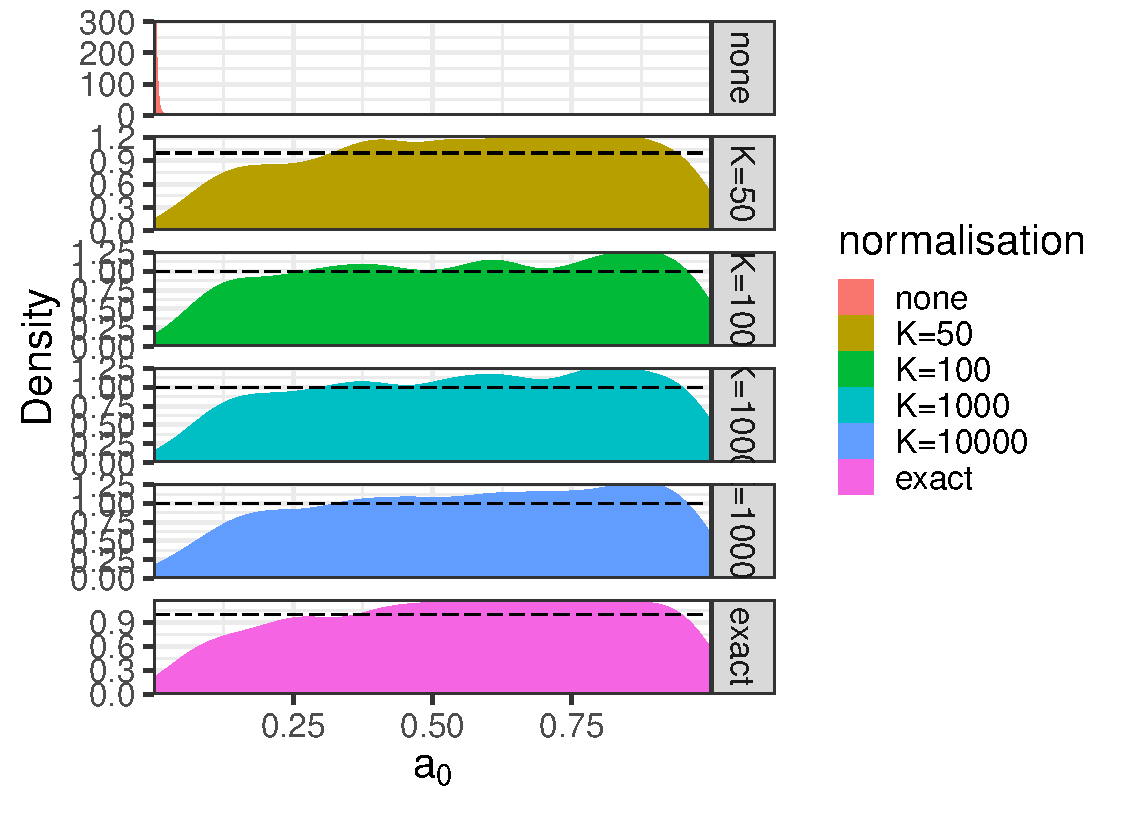
\includegraphics[width=7cm]{../figures/a0_posterior_Poisson.pdf}}
\hfill
\subfigure[$\lambda$]{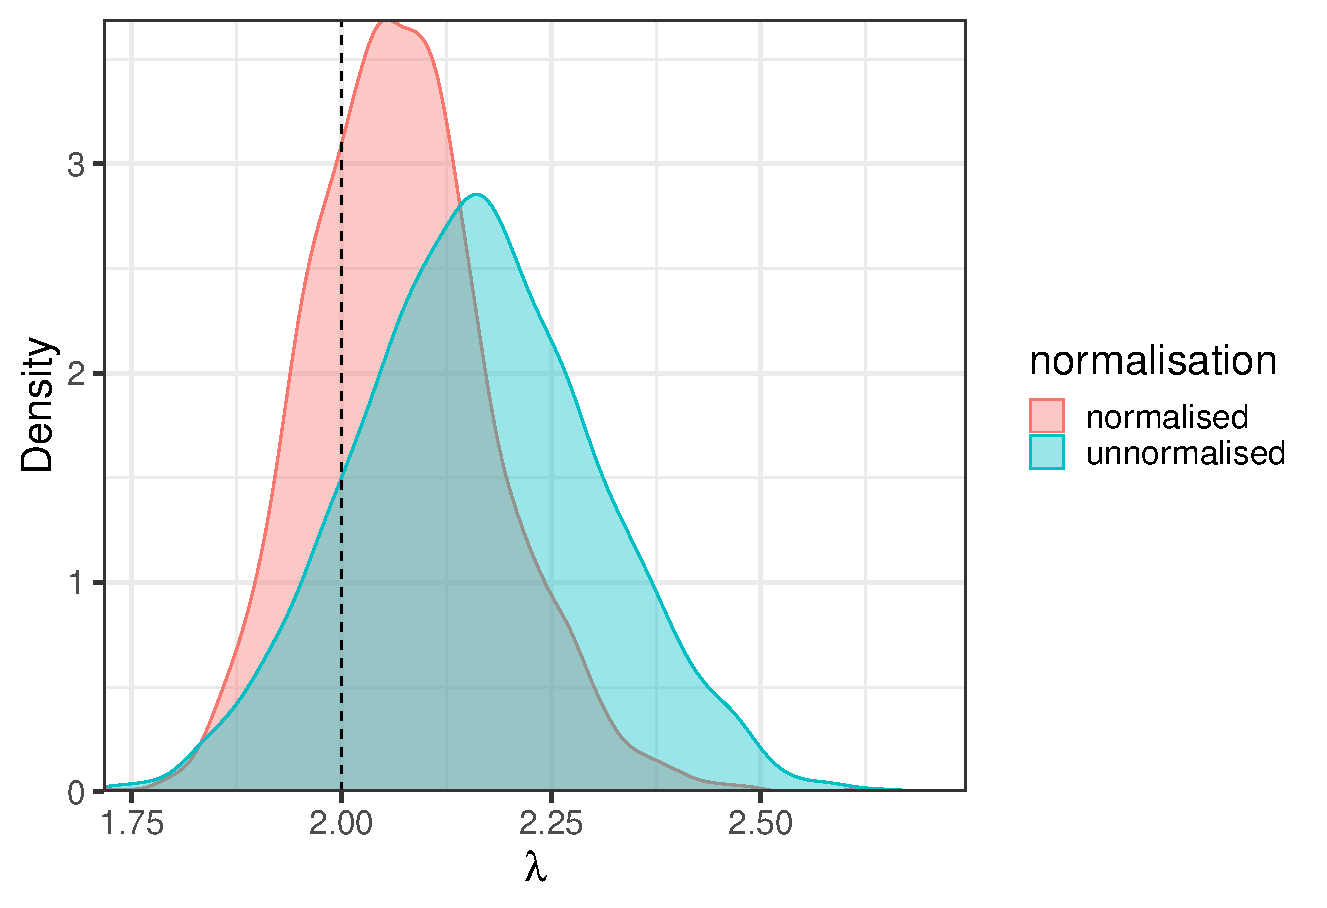
\includegraphics[width=7cm]{../figures/parameter_posterior_Poisson.pdf}}
\hfill
\caption{\textbf{Results for the Poisson example}.
Panels (and colours) correspond to various values of the approximation grid, $K$, as well as the results with no normalisation.
In panel (a) we show the marginal posterior for $a_0$, using horizontal dashed lines to show the prior density of a $\text{Beta}(\eta = 1, \nu = 1)$.
}
\label{fig:poisson}
\end{figure}

\subsection{Gaussian likelihood with unknown mean and variance}
\label{sec:gaussian_illus}

Now we move on to study a case where $c(a_0)$ is non-monotonic and thus presents a more challenging setting.
Suppose one has $N_0$ historical observations $y_{i0} \in \mathbb{R}, i = 1, \ldots, N_0$, which come from a Gaussian distribution with parameters $\mu$ and $\tau$.
Here we will choose a normal-Gamma conjugate model:
\begin{align*}
 \tau &\sim \text{Gamma}(\alpha_0, \beta_0),\\
 \mu &\sim \text{Normal}(\mu_0, \kappa_0\tau ),\\
 y_{0i} \mid \mu, \tau &\sim \text{Normal}(\mu, \tau),
\end{align*}
where the normal distribution is parametrised in terms of mean and precision (see below for a different parametrisation).
The posterior distribution is again a normal-Gamma distribution and the normalising constant is
\begin{align}
 \label{eq:cA0_gaussian}
 c(a_0) &= \frac{\Gamma(\alpha_n)}{\Gamma(\alpha_0)}\frac{\beta_0^{\alpha_0}}{\beta_n^{\alpha_n}} \left(\frac{\kappa_0}{\kappa_n} \right)^2 (2\pi)^{-N_0 a_0/2},\\
 \nonumber
 \alpha_n &= \alpha_0 + \frac{1}{2}a_0N_0, \\
 \nonumber
 \kappa_n &= \kappa_0 + a_0N_0, \\
 \nonumber
 \beta_n  &= \beta_0 + \frac{1}{2}\left( a_0\sum_{i=1}^{N_0}(y_{0i}-\bar{y})^2 + \left(\kappa_0 a_0 N_0 (\bar{y}-\mu_0)^2\right)/\kappa_n \right),
\end{align}
with $\bar{y} = N_0^{-1}\sum_{i=1}^{N_0} y_{0i}$.
In Appendix~\ref{sec:ca0_norm_deriv}, we give a closed-form expression for $c^\prime(a_0)$ and characterise the point of inflection of $c(a_0)$ by giving the conditions for $c^\prime(a_0) = 0$.

To make things concrete, we generate $N_0 = 50$ data points from a Gaussian distribution with parameters $\mu = -0.1$ and  $\tau = 10^{6}$.
We construct the Gamma prior on $\tau$ with $\alpha_0 = \beta_0 = 1$ and assign a Gaussian prior on $\mu$, with parameters $\mu_0 = 0$ and $\kappa_0 = 5$.
This
% admittedly odd
choice of hyperparameters leads to a function $c(a_0)$ -- Equation~(\ref{eq:cA0_gaussian}) -- that resembles a concave up parabola (Figure~\ref{fig:gaussian_results}a). 
We then generate $N = 20$ new points from the same distribution to be used as current data.
The points show the values of $l(a_0)$ and $l^\prime(a_0)$ estimated using the algorithm described in Section~\ref{sec:adapt_grid}, which exploits the derivatives of $c(a_0)$ to place more points closer to the region where $c^\prime(a_0)$ (and $l^\prime(a_0)$) changes signs.

We show the resulting marginal posteriors for $\mu$ and $\tau$ as well as $a_0$ under no normalisation, exact and approximate normalisation with various $K$ in Figure~\ref{fig:gaussian_results}b and~\ref{fig:gaussian_results}c.
The first observation is that approximations with $K > 100$ seem to produce marginal posteriors for $a_0$ that resembles the exactly normalised distribution quite closely, even in this setting, where $c(a_0)$ is non-linear.

In terms of parameter posteriors, we find that the posterior is not very sensitive to the value of $a_0$, as shown by the overlap between marginal posteriors with no normalisation as well as exact and approximate normalisation.
Even in this setting the approximately normalised marginal posteriors match their exact counterparts closely.

\begin{figure}[!ht]
\hfill
\subfigure[(log) normalising constant ]{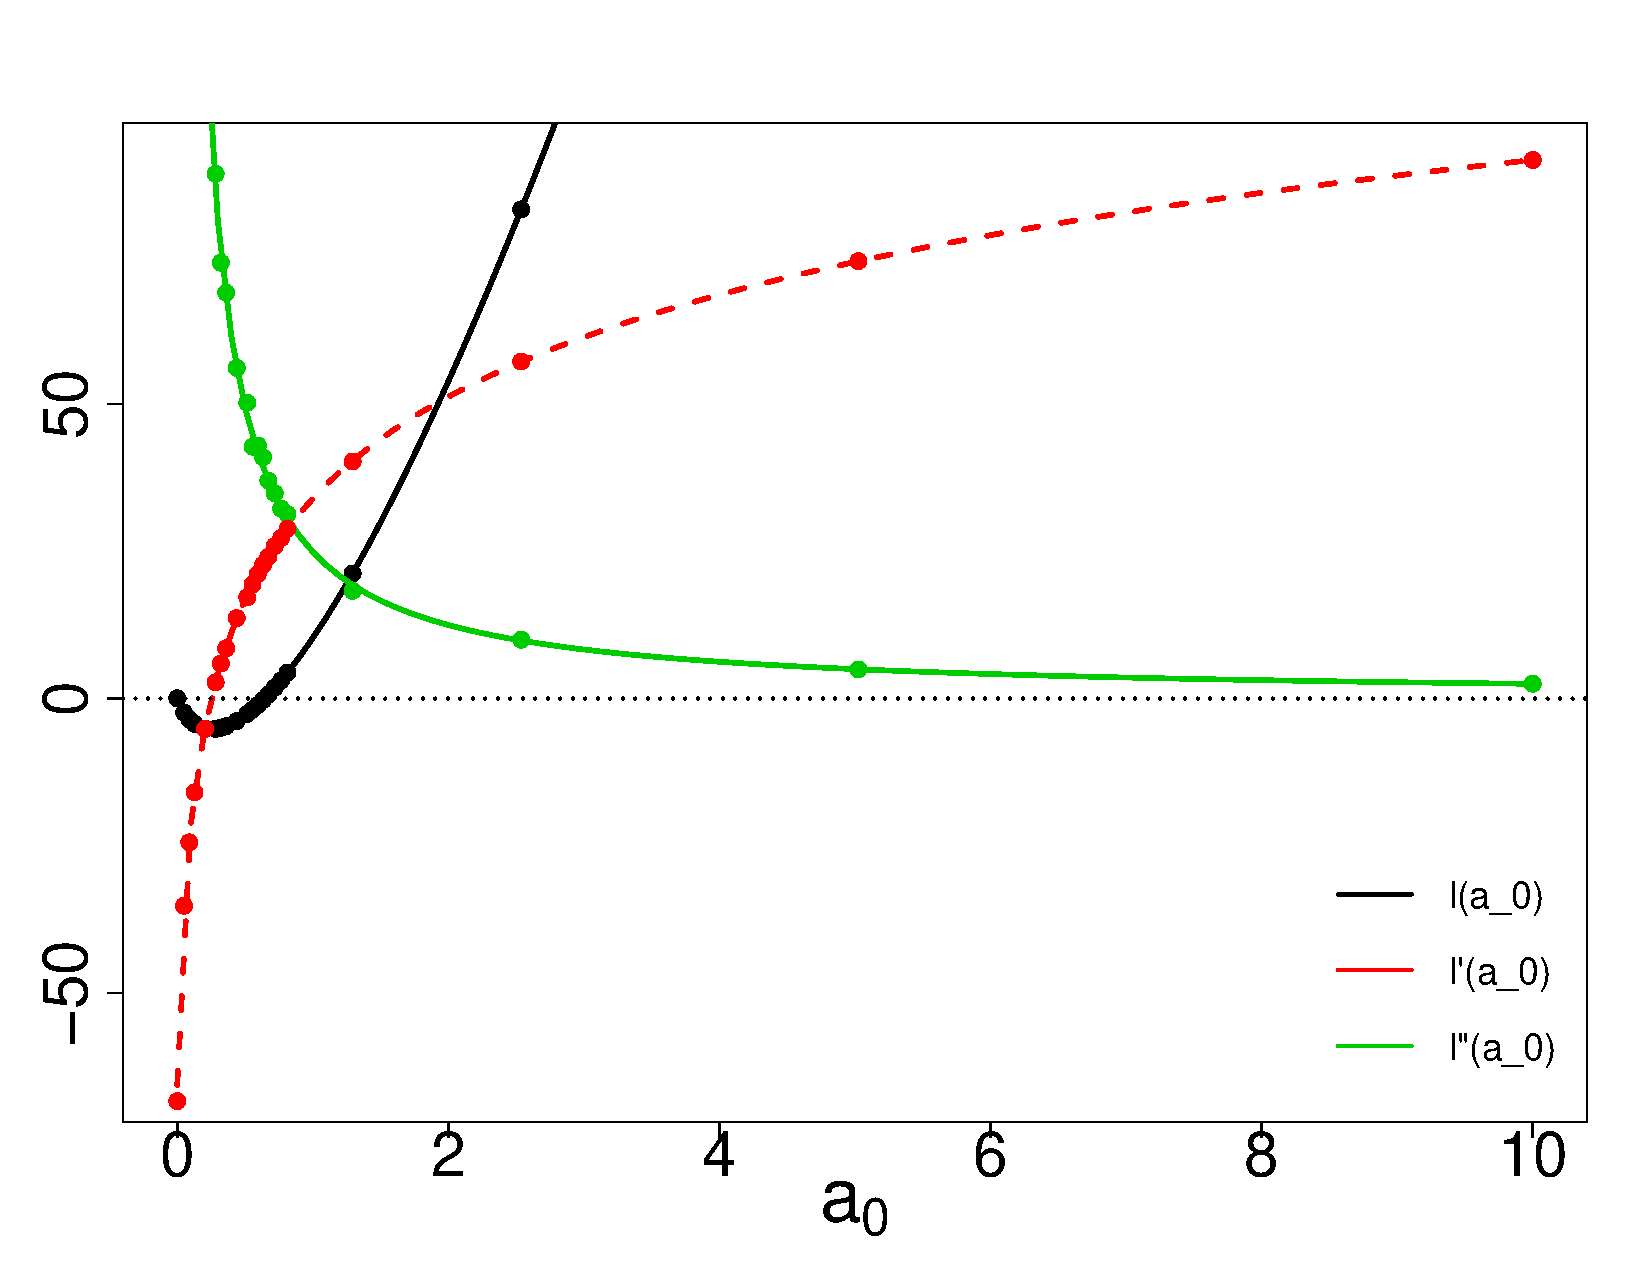
\includegraphics[width=7cm]{../figures/Gaussian_curves.pdf}}
\hfill
\subfigure[$a_0$ posterior]{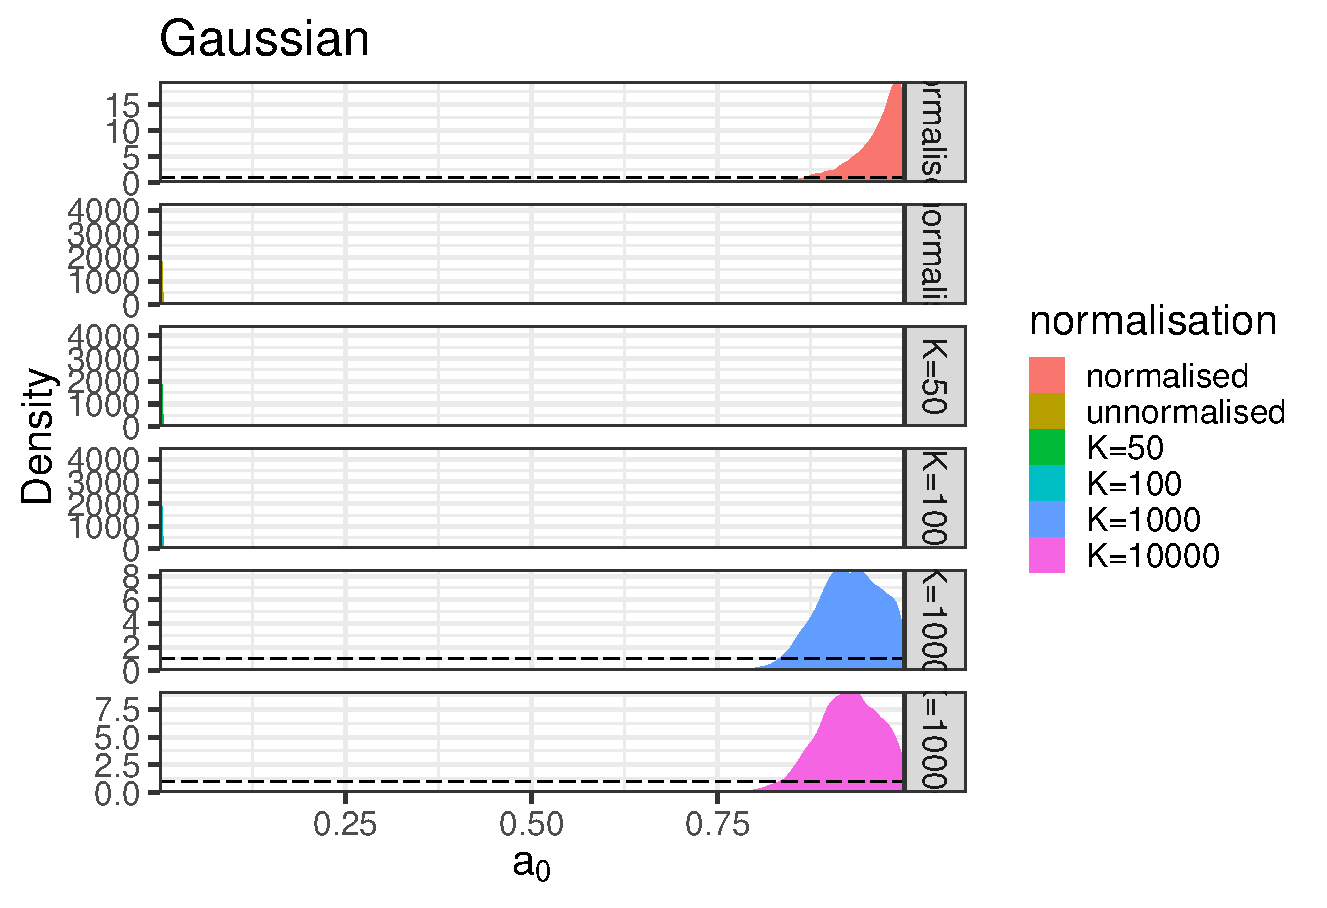
\includegraphics[width=7cm]{../figures/a0_posterior_Gaussian.pdf}}\\
\hfill
\subfigure[Parameter posteriors]{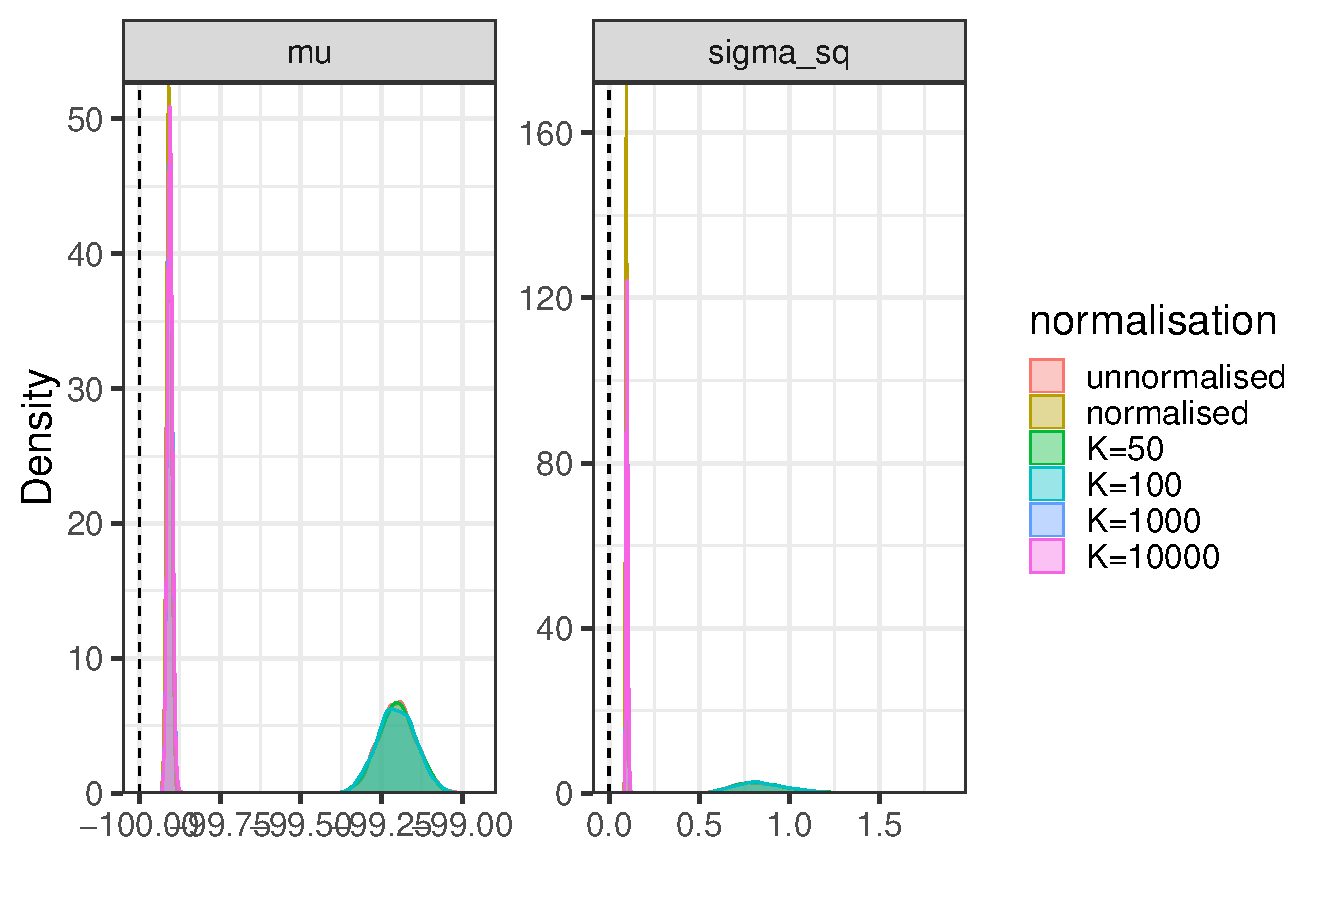
\includegraphics[width=7cm]{../figures/parameter_posterior_Gaussian.pdf}}
\hfill
\caption{\textbf{Results for the Gaussian example}.
In panel (a) we show $l(a_0) := \log(c(a_0))$ and its first two derivatives.
Points show the $J = 20$ estimates of $l(a_0)$ and $l^\prime(a_0)$ obtained using the algorithm in Section~\ref{sec:adapt_grid}.
In panel (b)  we show the marginal posterior of $a_0$ under no normalisation, exact normalisation or approximate normalisation with various grid sizes ($K$) in each subpanel.
Horizontal dashed lines show the prior density of a $\text{Beta}(\eta = 1, \nu = 1)$.
In (c) we show the marginal posteriors for $\mu$ and $\tau$ under no normalisation, exact normalisation or approximate normalisation with various grid sizes ($K$) in each subpanel.
}
\label{fig:gaussian_results}
\end{figure}

We also evaluate the performance of adaptively building the grid of $a_0$ by comparing the mean absolute error (MAD) and root mean squared error (RMSE) of the estimated function $g_{\hat{\xi}}$ to the true (exact) normalisation when using either a uniform grid or the adaptive grid.
Over the whole range of $a_0 \in [0, 10]$ we found that the uniform grid leads to an estimated function with lower MAD ($0.59$ vs $0.82$) and lower RMSE ($0.99$ vs $1.18$). 
When considering only the range $a_0 \in [0, 1]$, the support of the prior -- $\pi_A(a_0)$ --,  we find the opposite: the adaptive grid outperforms uniform with MAD $2.10$ vs $0.10$ and RMSE $2.73$ vs $0.13$.
This suggests that the adaptive scheme would produce better results in situations where the region where the derivative changes lies within the support of the prior.

\subsubsection{Linear regression with a normal inverse-Gamma prior}
\label{sec:linreg_ex}
To conclude the examples for which we know $c(a_0)$ in closed-form, we present a popular model for Bayesian linear regression.
Suppose $\boldsymbol X_0$ is a $N_0 \times P$ full-rank matrix of predictors and $\boldsymbol y_0 = \{y_{01}, \ldots, y_{0N_0} \}$ is a vector of observations.
For illustrative purposes, we will employ a mean and variance parametrisation, which naturally leads to a normal inverse-Gamma conjugate prior.
The model is 
\begin{align*}
 \sigma^2 &\sim \text{Inverse-Gamma}(\alpha_0, \gamma_0),\\
 \epsilon_i \mid \sigma^2  &\sim \text{Normal}(0, \sigma^2), \\
 \beta \mid \sigma^2 &\sim \text{Normal}(\boldsymbol \mu_0, \sigma^2\boldsymbol\Lambda_0^{-1}),\\
 y_{0i} &= \boldsymbol X_{0i}^\top \boldsymbol\beta + \epsilon_i, \\
\end{align*} 
where $\boldsymbol\beta$ is a $ 1 \times P$ vector of coefficients and $\boldsymbol\Lambda_0$ is a $P \times P$ variance-covariance matrix controlling the prior variance of the coefficients.
The posterior is again a normal inverse Gamma and thus
\begin{align}
 \label{eq:cA0_regression}
c(a_0) &= \sqrt{\frac{|\boldsymbol\Lambda_n|}{|\boldsymbol\Lambda_0^{-1}|}} \frac{\gamma_0^{\alpha_0}}{\gamma_n^{\alpha_n}}\frac{\Gamma(\alpha_0)}{\Gamma(\alpha_n)}  (2\pi)^{-N_0 a_0/2},\\
\nonumber
\boldsymbol\Lambda_n &= \boldsymbol X_{\star}^\top\boldsymbol X_{\star} + \boldsymbol \Lambda_0^{-1}, \\
\nonumber
\boldsymbol\mu_n &= \boldsymbol\Lambda_n^{-1}\left(\boldsymbol\Lambda_0^{-1}\boldsymbol\mu_0 + \boldsymbol X_{\star}^\top\boldsymbol y_{\star} \right),  \\
\nonumber
\alpha_n &= \alpha_0 + \frac{1}{2}a_0N_0,\\
\nonumber
\gamma_n &= \gamma_0 + \frac{1}{2}\left( \boldsymbol y_{\star}^\top \boldsymbol y_{\star} + \boldsymbol \mu_0^\top \boldsymbol \Lambda_0^{-1} \boldsymbol \mu_0 - \boldsymbol\mu_n^\top \boldsymbol \Lambda_n \boldsymbol \mu_n  \right),
\end{align}
where $\boldsymbol X_{\star} = \sqrt{a_0} \boldsymbol X_0$ and $\boldsymbol y_{\star} = \sqrt{a_0} \boldsymbol y_0$, and $|A|$ denotes the determinant of $A$.

We generate $N_0 = 1000$ data points, drawing the columns of $\boldsymbol X_0$ from a standard normal distribution and using $\boldsymbol \beta = \{ -1, 1, 0.5, -0.5\}$.
The response variable $Y_0$ is generated using a normal distribution with variance $\sigma^2 = 4$, i.e. $y_{0i} \sim \text{Normal}(\boldsymbol\beta^T \boldsymbol X_{0i}, 4)$.
For the current data, we generate $N = 100$ points using the same data-generating process.
To complete model specification we set $\alpha_0 = 1/2$, $\gamma_0 = 2$ and $\boldsymbol\Lambda_0 = \frac{3}{2}\boldsymbol I_P$, where $\boldsymbol I_P$ is the $P \times P$ identity matrix.

Results of the power prior analysis of this data are shown in Table~\ref{tab:results_NIGregression} and indicate that while parameter recovery is similar for the exactly normalised and approximately normalised posteriors, the approximate method does not recover the lower tail of the marginal posterior of $a_0$ well.
\begin{table}[!ht]
\label{tab:results_NIGregression}
\caption{\textbf{Parameter estimates for the linear regression example}.
We report the posterior mean and 95\% BCI for the regression parameters $\boldsymbol\beta$, response variance $\sigma^2$ and the power prior scalar, $a_0$.
We employed a  $\text{Beta}(\eta = \nu = 1)$ as prior for $a_0$.
}
{\small
\begin{tabular}{cccccc}
\hline 
 Parameter & True & None & Exact & app. $K = 50$ & app. $K = 10000$ \\
 \hline
$\beta_0$ & -1 & -0.56 (-0.98, -0.16) & -0.91 (-1.12, -0.59) & -0.92 (-1.12, -0.63) & -0.92 (-1.12, -0.68) \\
$\beta_1$ & 1 & 0.78 (0.38, 1.18) & 0.89 (0.66, 1.09) & 0.88 (0.69, 1.08) & 0.89 (0.67, 1.08) \\
$\beta_2$ & 0.5 & 0.32 (-0.05, 0.70) & 0.50 (0.24, 0.70) & 0.50 (0.28, 0.70) & 0.51 (0.29, 0.69) \\
$\beta_3$ & -0.5 & -0.68 (-1.04, -0.34) & -0.57 (-0.79, -0.39) & -0.58 (-0.78, -0.39) & -0.57 (-0.78, -0.38) \\
$\sigma^2$ & 4 & 3.7 (2.8, 4.8) & 4.4 (3.6, 5.0) & 4.4 (3.8, 5.1) & 4.4 (3.8, 5.0) \\
$a_0$ & -- & 0.00 (0.00, 0.00) & 0.48 (0.05, 0.97) &0.43 (0.11, 0.94) & 0.49 (0.09, 0.97)\\
\hline
\end{tabular}
}
\end{table}

\subsection{Logistic regression}
\label{sec:logistic_regression}

Next, we approach a problem for which $c(a_0)$ cannot be written in closed-form.
Logistic regression is very popular model for binary outcomes in the presence of explanatory variables (covariates). 
Taking $\boldsymbol Y_0 = \{y_{01}, y_{02}, \ldots, y_{0N_0} \}$ with $y_{0i} \in \{0, 1\}$ and a (assumed full rank) $N_0 \times P$ matrix of covariates $\boldsymbol X_0$ as historical data, the model we consider here is 
\begin{align*}
 y_{0i} &\sim \text{Bernoulli}(\theta_i), \\
 \theta_i &= \frac{\exp(\alpha + \boldsymbol X_{0i}^T \boldsymbol \beta)}{1 + \exp(\alpha + \boldsymbol X_{0i}^T \boldsymbol \beta)},\\
 \alpha & \sim \text{Normal}(0, 1), \\
 \beta_i &\sim \text{Normal}(0, 1),
\end{align*}
where $\alpha$ is the intercept and $\boldsymbol\beta$ is a $P$-dimensional vector of coefficients.
Since we do not have the benefit of a closed-form $c(a_0)$ in this example, we simulate data with known parameters and study how parameters are recovered as a function of the grid size $K$.
First, we generate $N_0 = 1000$ historical data points $(\boldsymbol Y_0, \boldsymbol X_0)$, where the matrix of covariates is constructed in the same manner as in the linear regression example.
We set $\alpha = 1.2$ and $\boldsymbol\beta = \{ -1, 1, 0.5, -0.5\}$.
For the current data, we use the same data-generating process to create a set of $N = 100$ new data points $(\boldsymbol Y, \boldsymbol X)$.
The chief idea is that a properly normalised power prior would allow one to capture the similarities between the historical and current data, while an analysis lacking the proper normalisation would yield counter-intuitive and suboptimal results, as demonstrated in the previous examples.
The results shown in Figure~\ref{fig:logistic_regression}a seem to support this intuition, since the approximately normalised power prior leads to posterior estimates that better recover the generating parameters, while the unnormalised prior leads to more diffuse posteriors that do not capture the full information contained in the data. 

\begin{figure}[!ht]
\hfill
\subfigure[Coefficients]{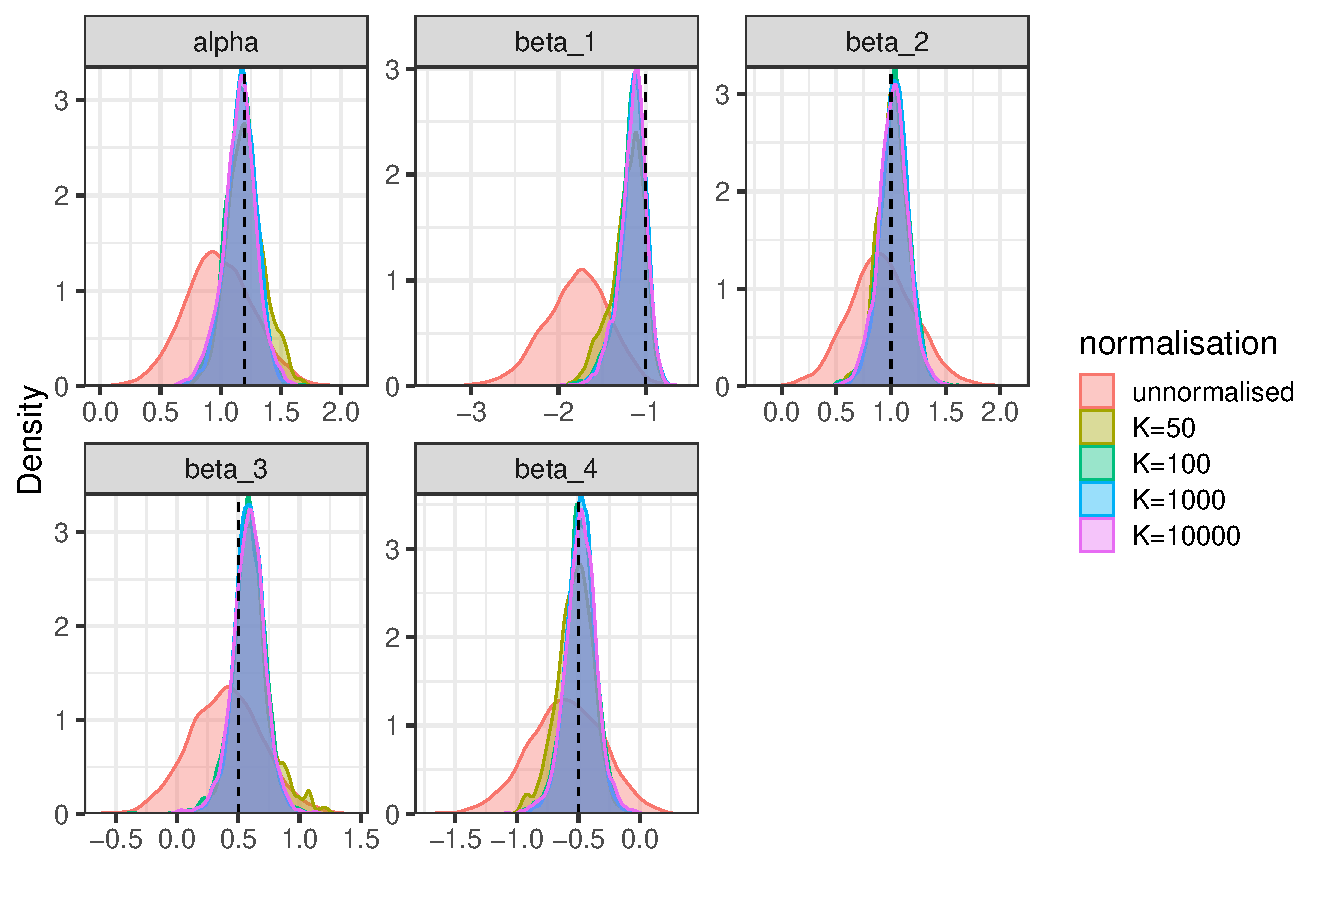
\includegraphics[width=7cm]{../figures/parameter_posterior_LogisticRegression.pdf}}
\hfill
\subfigure[$a_0$]{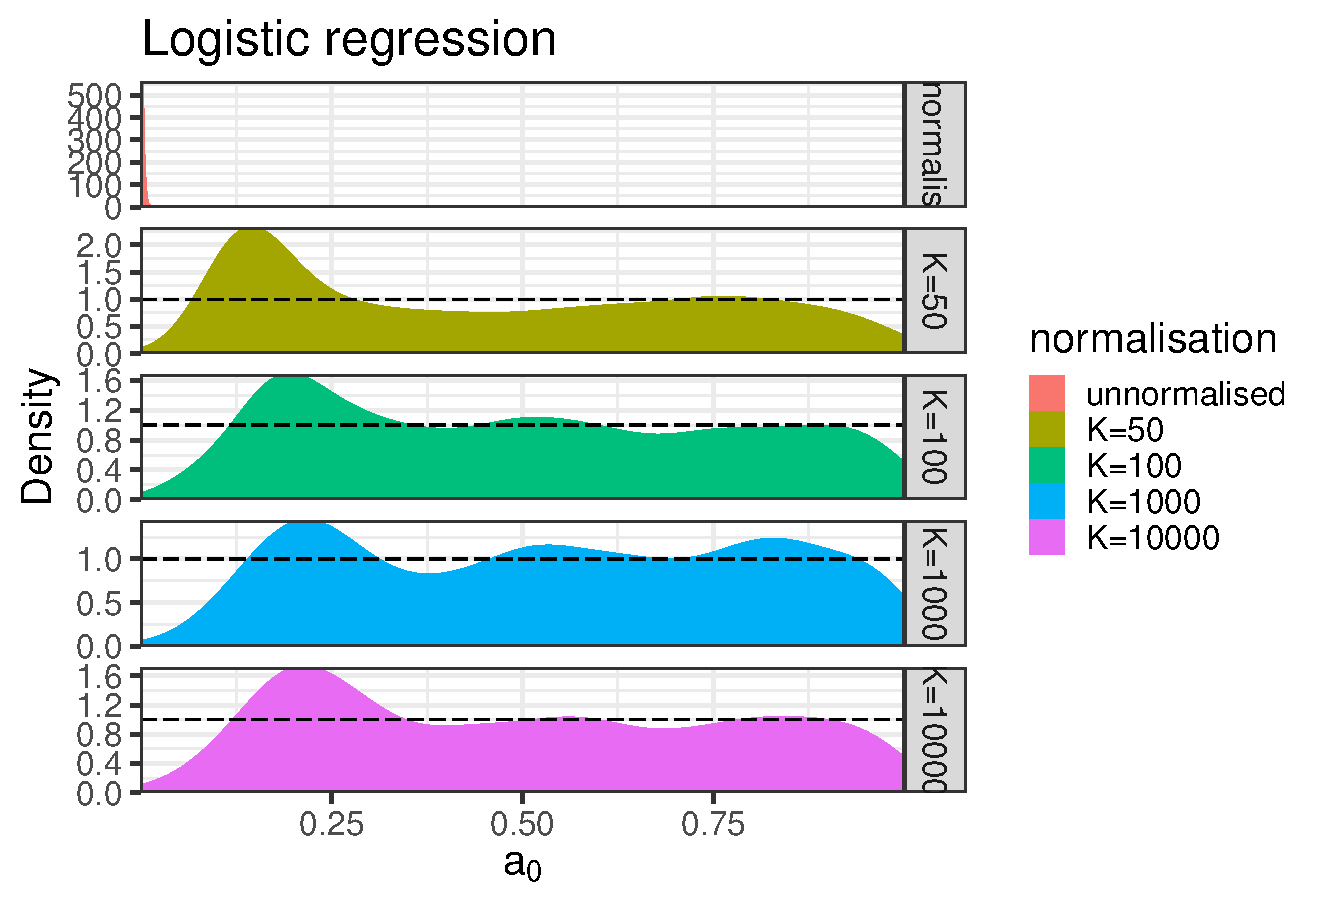
\includegraphics[width=7cm]{../figures/a0_posterior_RegressionLogistic.pdf}}
\hfill
\caption{\textbf{Results for the logistic regression example}.
Panel (a) shows the marginal posterior distributions for model parameters, with colours again pertaining to the approximation scheme.
Vertical dashed lines show the ``true'' parameter values of the data-generating process.
Horizontal dashed lines show the prior density of a $\text{Beta}(\eta = 1, \nu = 1)$.
In panel (b) the subpanels (and colours) correspond to the posterior distribution of the parameter $a_0$ when $c(a_0)$ is accounted for using various grid sizes $K$ and when it is not included.
}
\label{fig:logistic_regression}
\end{figure}

In addition we see that the approximate posteriors start to stabilize for $K > 1000$, showcasing the increased difficulty of this  multi-dimensional problem (see also Section~\ref{sec:linreg_ex}).
The bimodal marginal posterior for $a_0$ (Figure~\ref{fig:logistic_regression}b) 

\subsection{Survival model with cure fraction}
\label{sec:survival}

As a final illustration, we show an application of the approximation scheme to a complex survival model.

[DATA]

[MODEL]

% Please add the following required packages to your document preamble:
% \usepackage{multirow}
\begin{table}[!ht]
\caption{\textbf{Cure fraction rate model results}. ($K = 2E4$)}
\begin{tabular}{cccc}
\hline
                                            &           & \multicolumn{2}{c}{Estimates}                      \\ \hline
Prior on $a_0$, $\text{Beta}(\eta, \nu)$    & Parameter & Unnormalised         & App. Normalised  \\
\hline
\multirow{7}{*}{$\eta = 1$, $\nu  = 1$}     & Intercept & 0.10 (-0.11, 0.31)   & 0.47 (0.24. 0.70)           \\
                                            & Age       & 0.09 (-0.05,0.23)    & 0.15 (0.03, 0.26)           \\
                                            & Gender    & -0.13 (-0.44, 0.18)  & -0.31 (-0.48, -0.13)        \\
                                            & PS        & -0.23 (-0.76, 0.25)  & -0.04 (-0.33, 0.36)         \\
                                            & $\alpha$  & 1.30 (1.13, 1.48)    & 1.02 (0.93, 1.12)           \\
                                            & $\lambda$ & -1.36 (-1.63, -1.12) & -1.80 (-2.03, -1.55)        \\
                                            & $a_0$     & 0.00 (0.00, 0.00)    & 0.41 (0.19, 0.94)           \\
\multirow{7}{*}{$\eta = 50$, $\nu  = 50$}   & Intercept & 0.20 (-0.02, 0.44)   & 0.50 (0.29, 0.71)           \\
                                            & Age       & 0.10 (-0.04, 0.24)   & 0.15 (0.05, 0.26)           \\
                                            & Gender    & -0.17 (-0.44, 0.10)  & -0.33 (-0.49, -0.19)         \\
                                            & PS        & -0.19 (-0.72, 0.27)  & 0.07 (-0.25, 0.37)          \\
                                            & $\alpha$  & 1.17 (1.02, 1.32)    & 1.01 (0.92, 1.10)           \\
                                            & $\lambda$ & -1.47 (-1.75, -1.21) & -1.83 (-2.05, -1.62)        \\
                                            & $a_0$     & 0.03 (0.02, 0.04)    & 0.48 (0.37, 0.60)           \\
\multirow{7}{*}{$\eta = 100$, $\nu  = 100$} & Intercept & 0.28 (0.05. 0.52)    & 0.51 (0.29, 0.72)           \\
                                            & Age       & 0.11 (-0.02, 0.16)   & 0.16 (0.05, 0.26)           \\
                                            & Gender    & -0.20 (-0.43, 0.02)  & -0.33 (-0.49, -0.18)        \\
                                            & PS        & -0.15 (-0.61, 0.27)  & 0.07 (-0.27, 0.37)          \\
                                            & $\alpha$  & 1.11 (0.98, 1.24)    & 1.01 (0.92, 1.09)           \\
                                            & $\lambda$ & -1.56 (-1.84, -1.30) & -1.83 (-2.05, -1.63)        \\
                                            & $a_0$     & 0.07 (0.05, 0.08)    & 0.49 (0.42, 0.56)           \\
\multirow{7}{*}{$\eta = 200$, $\nu  = 1$}   & Intercept & 0.38 (0.14, 0.63)    & 0.54 (0.36, 0.72)           \\
                                            & Age       & 0.13 (0.01, 0.25)    & 0.17 (0.09, 0.26)           \\
                                            & Gender    & -0.25 (-0.45, 0.06)  & -0.36 (-0.49, -0.24)        \\
                                            & PS        & -0.09 (-0.52, 0.31)  & 0.15 (-0.11, 0.39)          \\
                                            & $\alpha$  & 1.05 (0.93, 1.17)    & 1.00 (0.93, 1.07)           \\
                                            & $\lambda$ & -1.68 (-1.96, -1.48) & -1.89 (-2.06, -1.73)        \\
                                            & $a_0$     & 0.14 (0.12. 0.16)    & 1.00 (0.98, 1.00)           \\ \cline{2-4} 
\end{tabular}
\end{table}

% \section*{TODO:}
% \begin{itemize}
%   \item check derivation of conjugate exponential family result;
% \end{itemize}

% \section{Roadmap}
% The idea is to review and justify power priors for general regression models.
% Since the integral of~(\ref{eq:power_prior}) with respect to $\theta$ is quite complicated, it is nice and reassuring to know that it is computable, even we don't quite know how to compute it.
% So we need to
% \begin{itemize}
%  \item Review the necessary literature;
%  \item Write down a couple examples of interesting regression models: random effects and Cox model with right-censoring (cure rate/ promotion time model);
%  \item See if we can prove a few more interesting things about these models;
%  \item Show our general results and argue that they provide justification for general use of power priors: they can be normalised, even if sometimes it is very hard to do so.
%  \item Find and curate ``classic'' data sets and write some Stan code to fit the models above to them;
% \end{itemize}
% As I understand it currently, the paper would have review-y feel to it: review what has been done for regression models and then add some of new stuff we've figured out.

% \section{Questions}

% \begin{enumerate}
%  \item Is it not the case that when employing an unormalised power prior, we can't compute marginal likelihoods\footnote{What I mean to say here is that marginal likelihoods don't make any sense unless the prior is properly normalised.}? Does that matter in practice? LM: Yeah, you need a properly normalised prior.
%  \item Should we be pursuing ways of computing $c(a_0) := \int_{\boldsymbol \Theta} p(t \mid D, a_0)dt$ for general models? LM: YES!
% \item \textbf{The shape of $c(a_0)$}: From both a theoretical and practical point of view, it'd be nice to know when $c(a_0)$ is non-monotonic like for the Gaussian case [and a very special choice of hyperparameters] and when it's just a straight line, as for most models I've tested. 
% Appendix~\ref{sec:ca0_norm_deriv} contains some rudimentary analysis for the Gaussian case...
% \item \textbf{Exponential family}: it could be potentially fruitful to explore the results in Eq.~\ref{eq:expo_family_const} a bit more and maybe help answer the question above; under which conditions will a likelihood in the exponential family lead to a monotonic (and hence linear since we know it's definitely convex) $c(a_0)$?
% \item \textbf{Sensitivity to $a_0$}: (i) is this important? (ii)  how to define sensitivity? one thing to look at is variance reduction as $a_0 \to \infty$...
% At any rate, we know empirically that for some models (e.g. logistic regression) including the normalising constant is of utmost importance, whereas for others (e.g. Bernoulli), it doesn't seem to matter much.
% \textbf{Important:} When I say ``matters'' (or not), I'm talking about the effect on estimates of actual parameters, like regression coefficients or success probability.
% Including $c(a_0)$ always makes a HUGE difference for ``estimates'' of $a_0$, obviously.
% \item \textbf{Situations with $a_0 > 1$} Should we pursue this? It seems to me we should at least consider it, since we show that the power prior is proper for $a_0 > 1$ also.
% \end{enumerate}

\section{Discussion}
\label{sec:discussion}

Sensitivity to $a_0$: Bernoulli ain't much, logistic regression is more.

Gaussian example is artificial, for most settings $l(a_0)$ will be monotonic. 

Improvements: better approximating function (GP with first and second derivatives)

One might complain that $J=20$ is too much, but in a fixed power prior analysis one would also usually do a sensitivity analysis.


\section*{Acknowledgements}

The authors would like to thank Aditya Ravuri for pointing out the first part of the proof of Theorem 1. 
LMC would like to thank Leo Bastos (PROCC/Fiocruz) for helpful discussions, Dr. Beat Neuenschwander for clarifications regarding his paper and Chris Koenig for testing the computer code developed for this paper.
This study was financed in part by the Coordenação de Aperfeiçoamento de Pessoal de Nível Superior - Brasil (CAPES) Finance Code 001.
LMC is supported by a postodoctoral fellowship from CAPES.

\bibliography{../biblio/power_prior}

\appendix

\section{Bridge sampling}

\section{Additional results}
\label{sec:further_proofs}

\begin{proposition}
\label{prop:c_is_Cinfinity}
All of the derivatives of $c(a_0)$ exist, i.e., $c \in \mathcal{C}^{\infty}$.
\end{proposition}
\begin{proof}
First, we will assume that $L(D_0 \mid \theta) > 0\: \forall \theta \in \Theta$.
For covenience, let
\[  f(\theta) = \frac{L(D_0 \mid \theta)^{a_0} \pi(\theta)}{c(a_0)}. \]
Now, consider the change of variables $\theta \mapsto l$, with $l = \log(L(D \mid \theta))$.
Then we write
\[ h (l) = \frac{\exp(a_0 l) g(l)}{z(a_0)},\]
where $g(l)$ is a non-negative function that accomodates the transform $\theta \mapsto l$ with respect to the prior $\pi$ and $z(a_0)$ is the appropriate normalsing constant, guaranteed to exist by Theorem~\ref{thm:integrability}.
The moment-generating function (MGF) of $l$ is 
\[ M_t(l) = E_h[\exp(tl)] = \int_{-\infty}^\infty \frac{\exp((t + a_0) l) g(l)}{z(a_0)}\, dl.\]
Since $E_h[l^r] \equiv  \frac{d^r c(a_0)}{d a_0^r}$, all that remains is to show that $M_r(l)$ exists for all $r \geq 0$.
Under the change of variables discussed above, Theorem~\ref{thm:integrability} shows that
\[ \int_{-\infty}^\infty \exp(wl) g(l)\, dl < \infty,\]
for $w > 0$.
Making $w = t + a_0$ concludes the proof.
\end{proof}


\section{The derivative of $c(a_0)$ for the normal case}
\label{sec:ca0_norm_deriv}
Define
\begin{align*}
 c(a_0) &= g(a_0)h(a_0)w(a_0)z(a_0), \\
 g(a_0) &:=  \frac{\Gamma\left( \alpha_0 + \frac{N_0}{2}a_0 \right)}{\Gamma(\alpha_0)}, \\
 h(a_0) &:= \frac{\beta_0^{\alpha_0}}{ \left(  \beta_0 + \Delta a_0\right)^{\alpha_0 + \frac{N_0}{2}a_0}}, \\
 w(a_0) &:= \left(\frac{\kappa_0}{\kappa_0 + N_0 a_0} \right)^2 , \\
 z(a_0) &:= (2\pi)^{-N_0 a_0/2}, 
\end{align*}
with $\Delta =  \frac{1}{2}\left( \sum_{i=1}^{N_0}(y_{0i}-\bar{y})^2 + \frac{\kappa_0}{\kappa_n} N_0 (\bar{y}-\mu_0)^2 \right)$.
Thus, dropping dependency on $a_0$ for notational compactness, we have
\begin{equation}
\label{eq:c_deriv_gaussian}
 c^\prime = h w z g^\prime + g w z h^\prime + g h z w^\prime + g h w z^\prime.
\end{equation}
Notice that only the first term of~(\ref{eq:c_deriv_gaussian}) is positive.
Since $g^\prime(a_0) = \frac{N_0}{2} \psi_0\left( \alpha_0 +  \frac{N_0}{2} a_0 \right)g(a_0)$, we can write the following inequality:
\begin{equation}
 c^\prime(a_0) > 0 \implies \frac{N_0}{2} \psi_0\left( \alpha_0 +  \frac{N_0}{2} a_0 \right) > \frac{|h^\prime(a_0)|}{h(a_0)} + \frac{|w^\prime(a_0)|}{w(a_0)} + \frac{|z^\prime(a_0)|}{z(a_0)}.
\end{equation}
Since
\begin{align}
 \frac{|h^\prime(a_0)|}{h(a_0)}  &=  \frac{\Delta\left( \alpha_0 + \frac{N_0}{2} a_0 \right) }{\Delta a_0 + \beta_0} + \frac{N_0}{2}\log{\left( \Delta a_0+ \beta_0 \right) }, \\
 \frac{|w^\prime(a_0)|}{w(a_0)}  &= \frac{2N_0}{a_0N_0+\kappa_0},\\
\frac{|z^\prime(a_0)|}{z(a_0)}  &= \log(2\pi) \frac{N_0}{2},
\end{align}
we arrive at
\begin{align}
 \frac{N_0}{2} \psi_0\left( \alpha_0 +  \frac{N_0}{2} a_0 \right) &>  \frac{\Delta\left( \alpha_0 + \frac{N_0}{2} a_0 \right) }{\Delta a_0 + \beta_0} + \frac{N_0}{2}\log{\left( \Delta a_0+ \beta_0 \right) } + \frac{2N_0}{a_0N_0+\kappa_0} + \log(2\pi) \frac{N_0}{2}, \\
\psi_0\left( \alpha_0 +  \frac{N_0}{2} a_0 \right) &>  \frac{\Delta\left( 2\alpha_0 + N_0a_0 \right) }{N_0\left(\Delta a_0 + \beta_0\right)} + \log{\left( \Delta a_0+ \beta_0 \right) } + \frac{4}{a_0N_0+\kappa_0} + \log(2\pi).
\end{align}

\section{Comparing approximations of $l(a_0)$}
\label{sec:derivative_only}

In this section we study two approaches to estimating $l(a_0)$, using four examples where it is known in closed-form.
First, we consider the main approach discussed in this paper, which consists of estimating $l(a_0)$ at a grid of $J = 15$ points of $a_0$ and using a GAM as the approximating function $g_\xi$ to approximate $l(a_0)$ directly.
We then evaluate the fitted function at a grid of $K = 20,000$ values to form a vector $\boldsymbol l_{\text{direct}}$.

Another approach is to use estimates of $l^\prime(a_0)$ (see Equation~\ref{eq:derivative_ca0}) as data and fit a GAM as the approximating function $h_\omega$ and evaluate this function at a fine grid of values for $a_0$.
We can then approximate $l(a_0)$ by midpoint integration, forming a vector of predictions/estimates $\boldsymbol l_{\text{deriv}}$.
Other methods, such as trapezoid integration might also be used.
We then compare the estimated values with the true values, $\boldsymbol l_{\text{true}}$, by computing the root mean squared error, $\hat{r} = \sqrt{\frac{1}{K} \sum_{i= 1}^K \left( l^{(i)}_{\text{est}} - l^{(i)}_{\text{true}} \right)^2 }$.

We show results for the Bernoulli, Poisson, Gaussian and linear regression in Table~\ref{tab:rmse_approx}.
Results are presented for two values of the $a_0$ endpoint, $M = 1$ and $M = 10$.
As expected, estimates (predictions) derived using direct estimation of $l(a_0)$ are substantially more accurate.
The only instance in which the derivative-based method is more accurate is for the Gaussian model and for a large endpoint $M = 10$.
Of the four models considered, only the Gaussian example (see section~\ref{sec:gaussian_illus}) has a non-monotonic $l(a_0)$, which might explain the observed results.

\begin{table}[!ht]
\caption{\textbf{ Mean root squared error comparison of methods for approximating $l(a_0)$}.
We used $J = 15$ points to construct $\boldsymbol a^{\text{est}}$ and use a GAM to approximate either $l(a_0)$ or $l^\prime(a_0)$. 
In the latter case, we evaluate the fitted function on a fine grid ($K = 20, 000$ points) and obtain an approximation of $l(a_0)$~\textit{via} midpoint integration (see text).
}
\begin{center}
\label{tab:rmse_approx}
\begin{tabular}{ccccc}
\hline
        Model          & \multicolumn{2}{c}{$M = 1$} & \multicolumn{2}{c}{$M = 10$} \\
\hline
                  & Direct & Deriv + midpoint & Direct  & Deriv + midpoint \\
Bernoulli         & 0.08   & 1.61             & 0.17    & 1.03             \\
Poisson           & 0.05   & 1.02             & 0.13    & 1.97             \\
Linear regression & 0.33   & 6.33             & 0.71    & 7.06             \\
Gaussian          & 1.74   & 10.08            & 31.29   & 12.11           \\
\hline
\end{tabular} 
\end{center}
\end{table}

% \begin{figure}[!ht]
% \centering
% \includegraphics[width=\textwidth, height = 15cm]{figures/}
% \caption{\textbf{}.
% }
% \label{fig:}
% \end{figure}
%%
% \newpage
% \begin{figure}
% \hfill
% % 
% \subfigure[Gaussian]{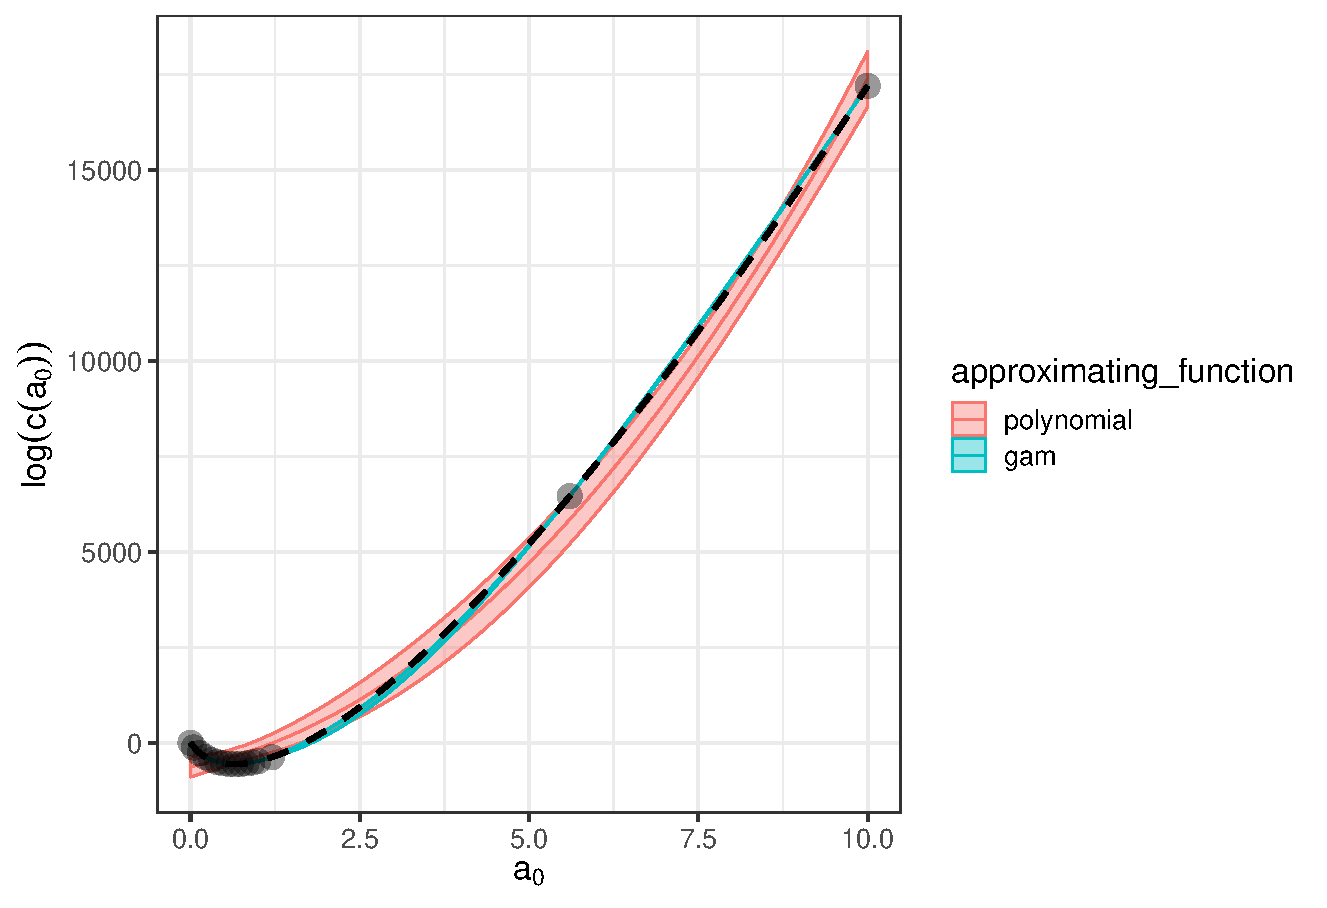
\includegraphics[width=7cm]{../figures/estimates_log_ca0_Gaussian.pdf}}
% \hfill
% \subfigure[Inverse-Gaussian]{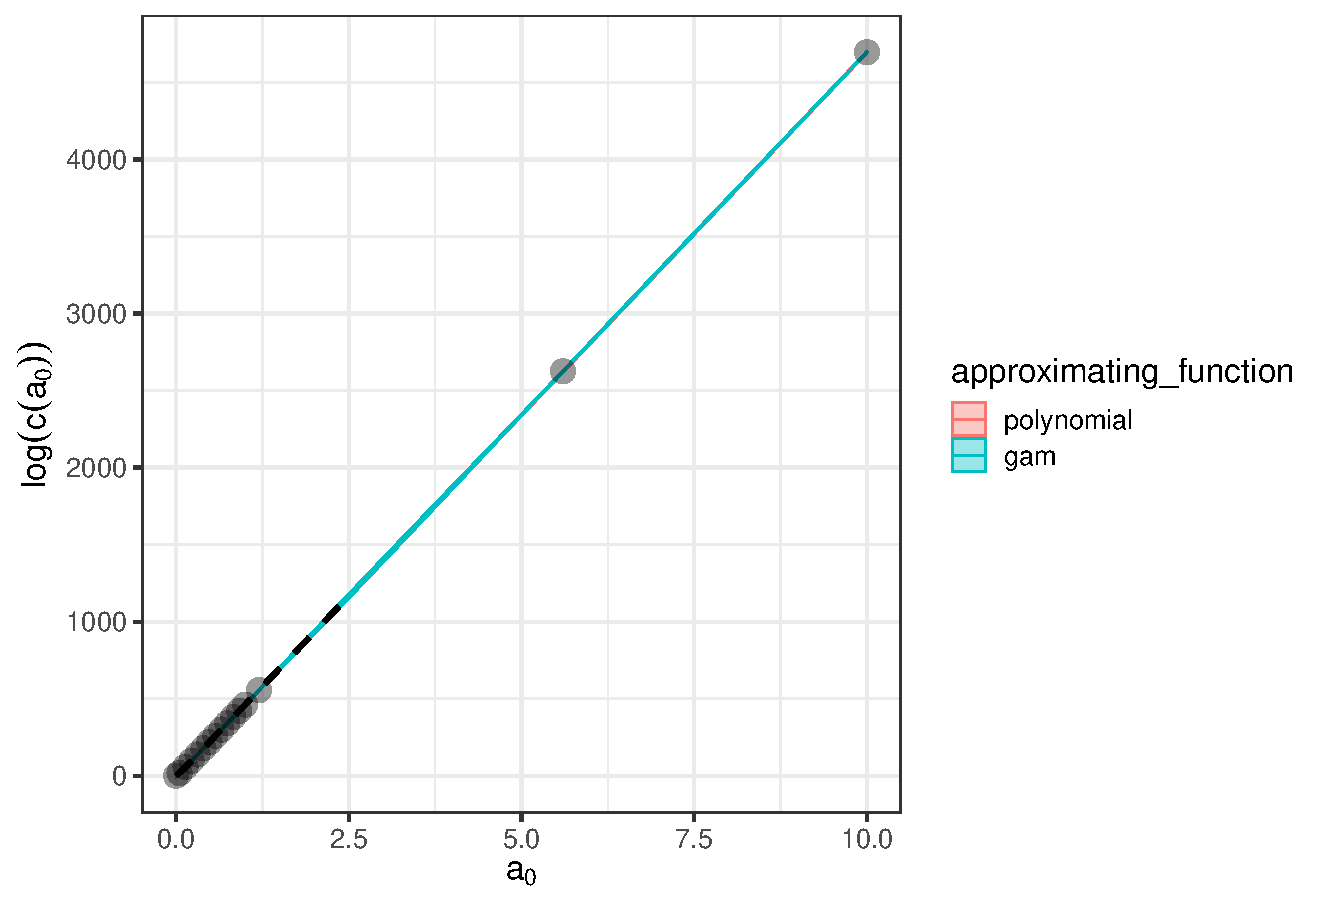
\includegraphics[width=7cm]{../figures/estimates_log_ca0_invGaussian.pdf}}\\
% \hfill
% \subfigure[Linear regression]{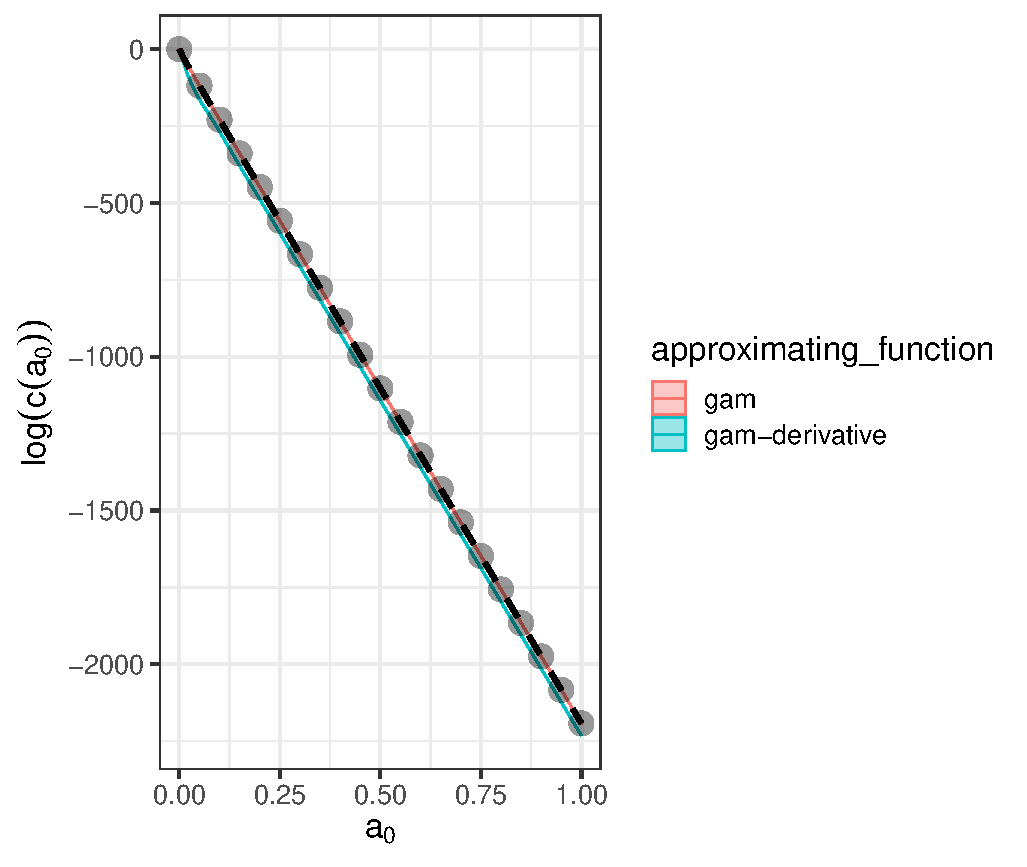
\includegraphics[width=7cm]{../figures/estimates_log_ca0_RegressionNIG.pdf}}
% \hfill
% \subfigure[Logistic regression]{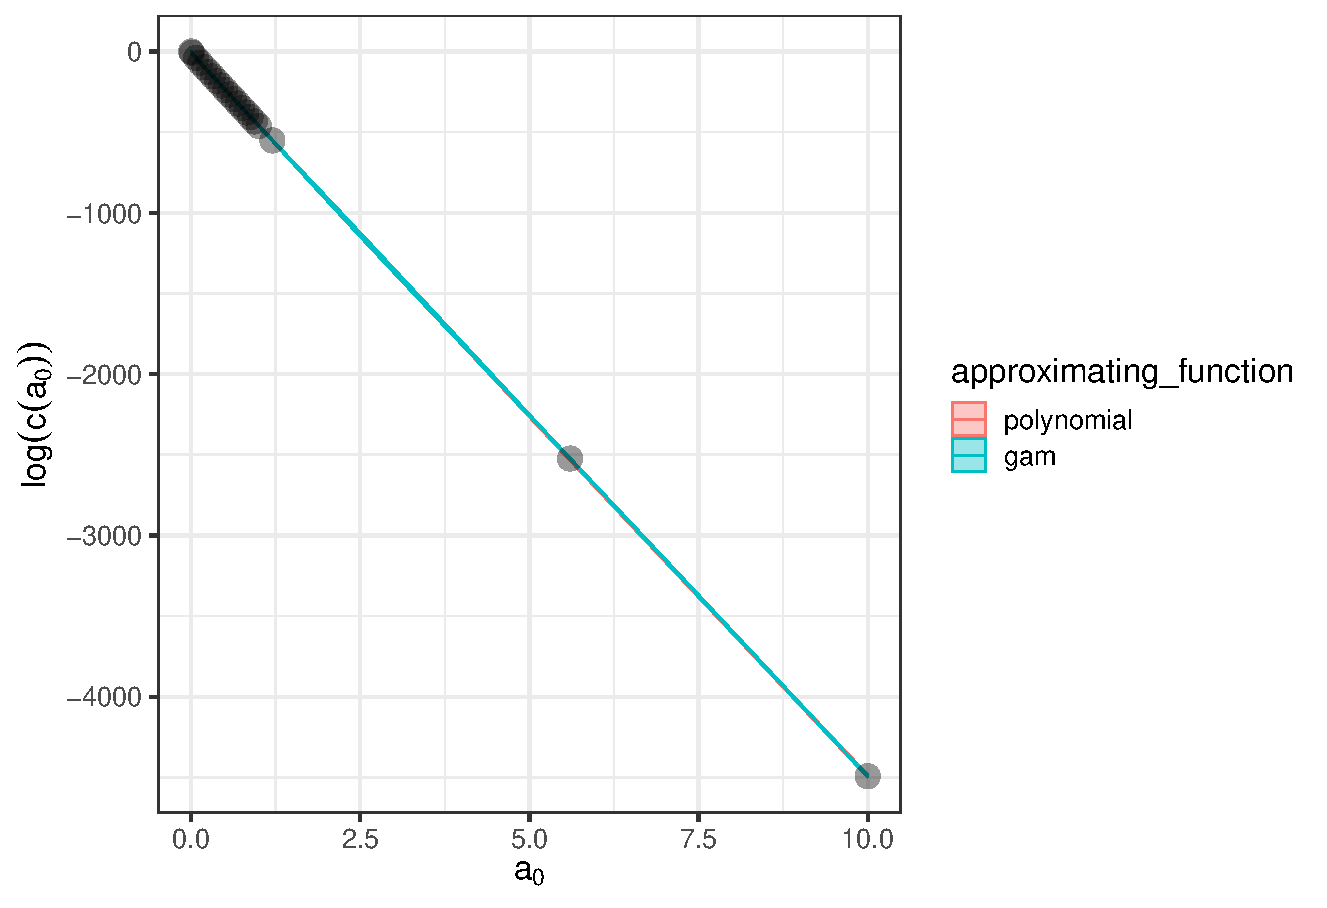
\includegraphics[width=7cm]{../figures/estimates_log_ca0_RegressionLogistic.pdf}}
% 
% \caption{\textbf{The normalising constant $c(a_0)$ for several models}.
% The plots show $\log c(a_0)$ for a host of models.
% Notice how for the inverse-Gaussian model  $\log c(a_0)$ is~\textbf{increasing} in $a_0$.
% Dashed line shows the true $c(a_0)$, when it exists or can be computed.
% }
% \label{fig:cA0}
% \end{figure}

% \begin{figure}
% \hfilly
% \subfigure[Gaussian]{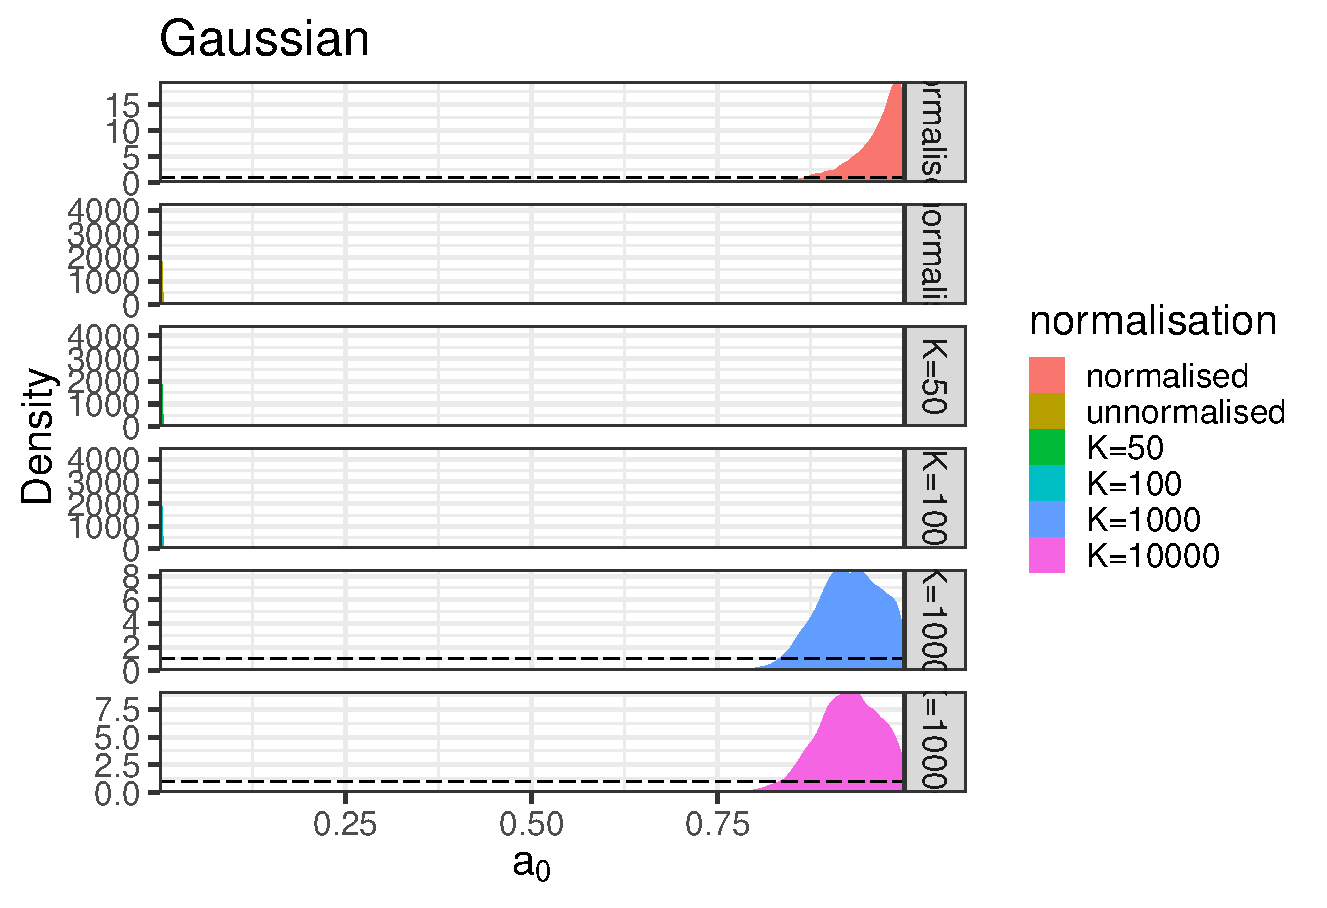
\includegraphics[width=7cm]{../figures/a0_posterior_Gaussian.pdf}}
% \hfill
% \subfigure[Inverse-Gaussian]{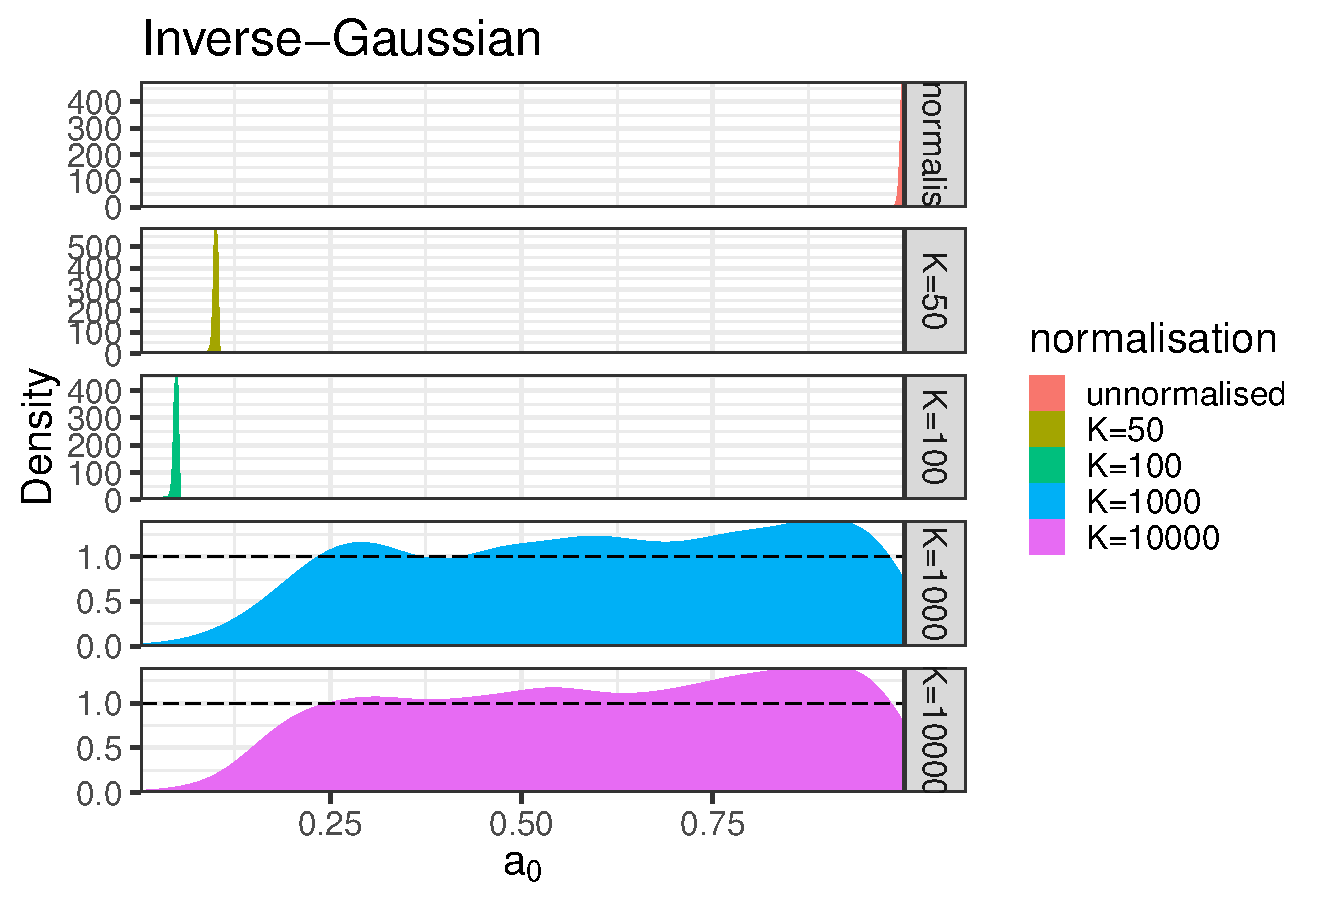
\includegraphics[width=7cm]{../figures/a0_posterior_invgaussian.pdf}}\\
% \hfill
% \subfigure[Linear regression]{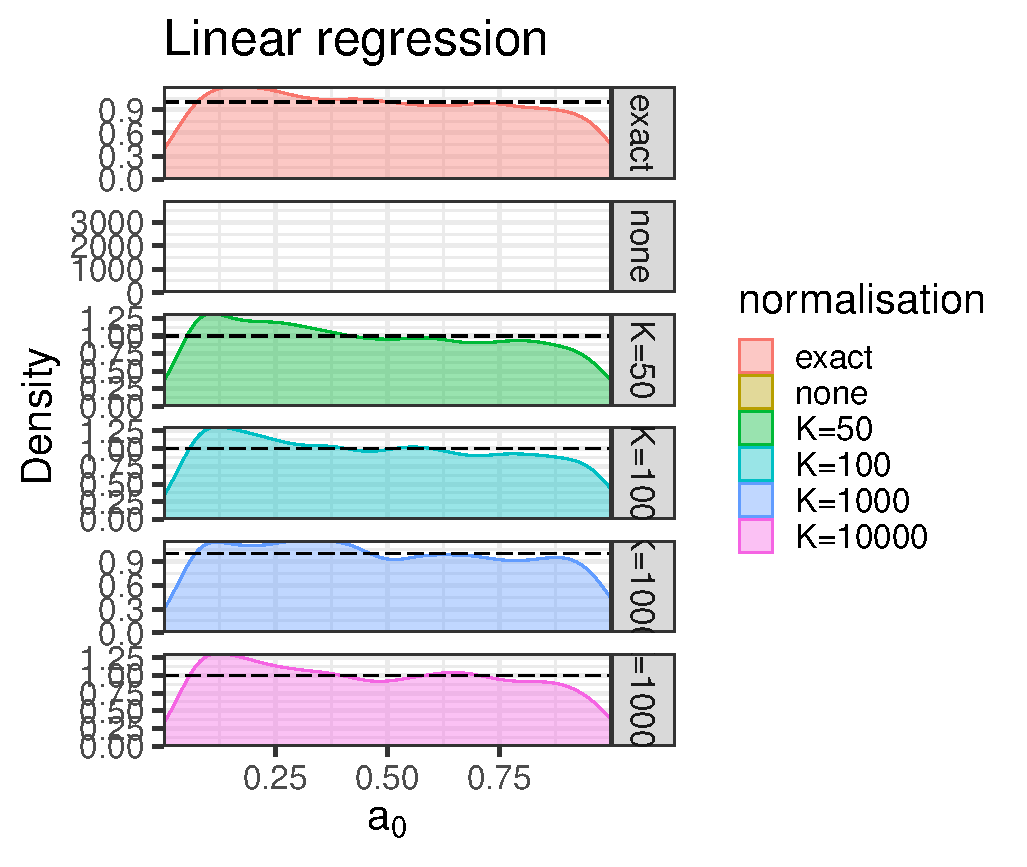
\includegraphics[width=7cm]{../figures/a0_posterior_RegressionNIG.pdf}}
% \hfill
% \subfigure[Logistic regression]{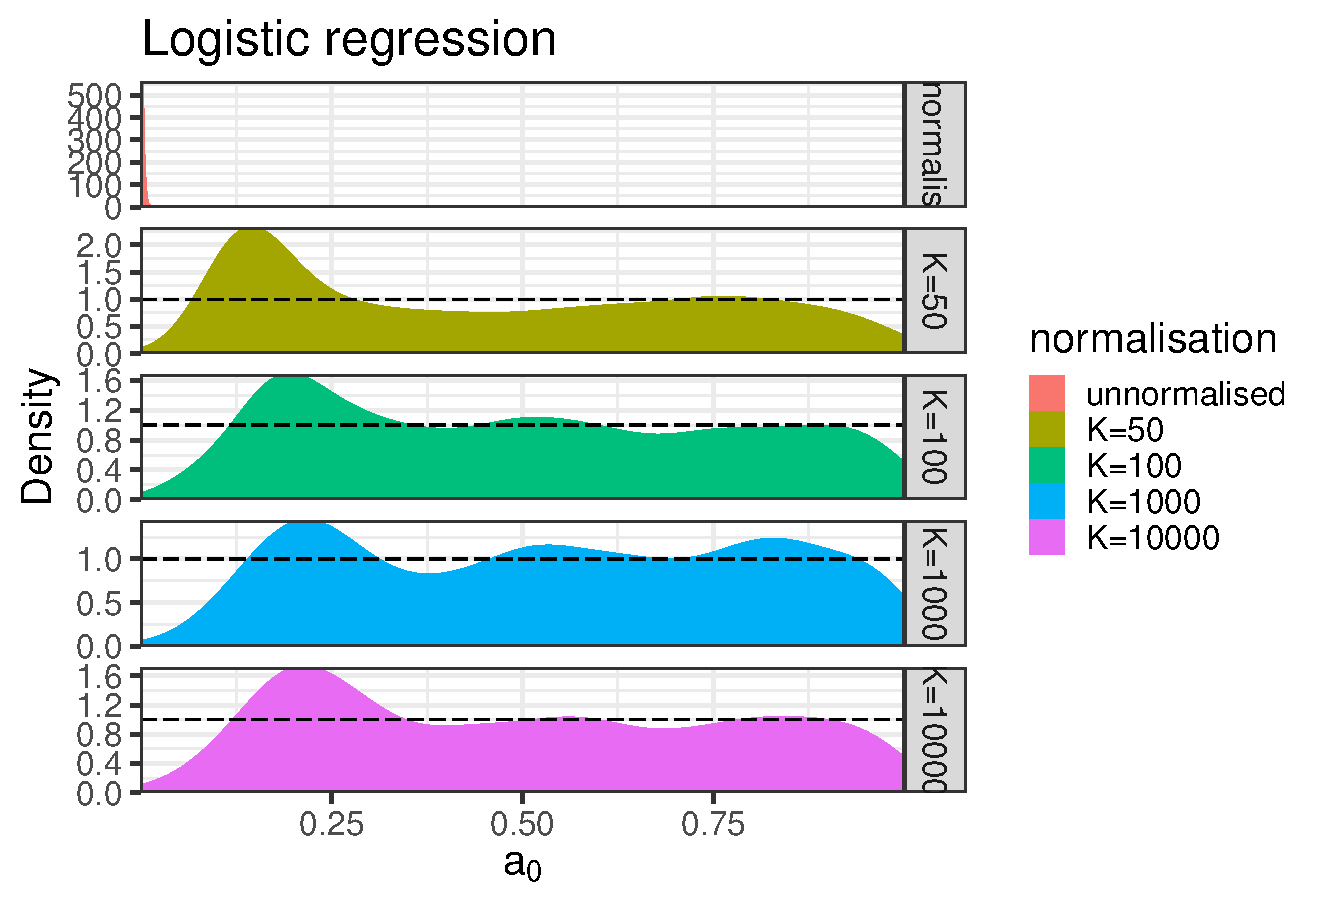
\includegraphics[width=7cm]{../figures/a0_posterior_RegressionLogistic.pdf}}
% \hfill
% \caption{\textbf{The posterior distribution of $a_0$ under normalised and unnormalised models}.
% The panels (and colours) correspond to the posterior distribution of the parameter $a_0$ when $c(a_0)$ is accounted for and when it is not included.
% Horizontal dashed lines show the prior density of a $\text{Beta}(\eta = 1, \nu = 1)$.
% }
% \label{fig:normalisation}
% \end{figure}

% \begin{figure}
% \hfill
% \subfigure[Gaussian]{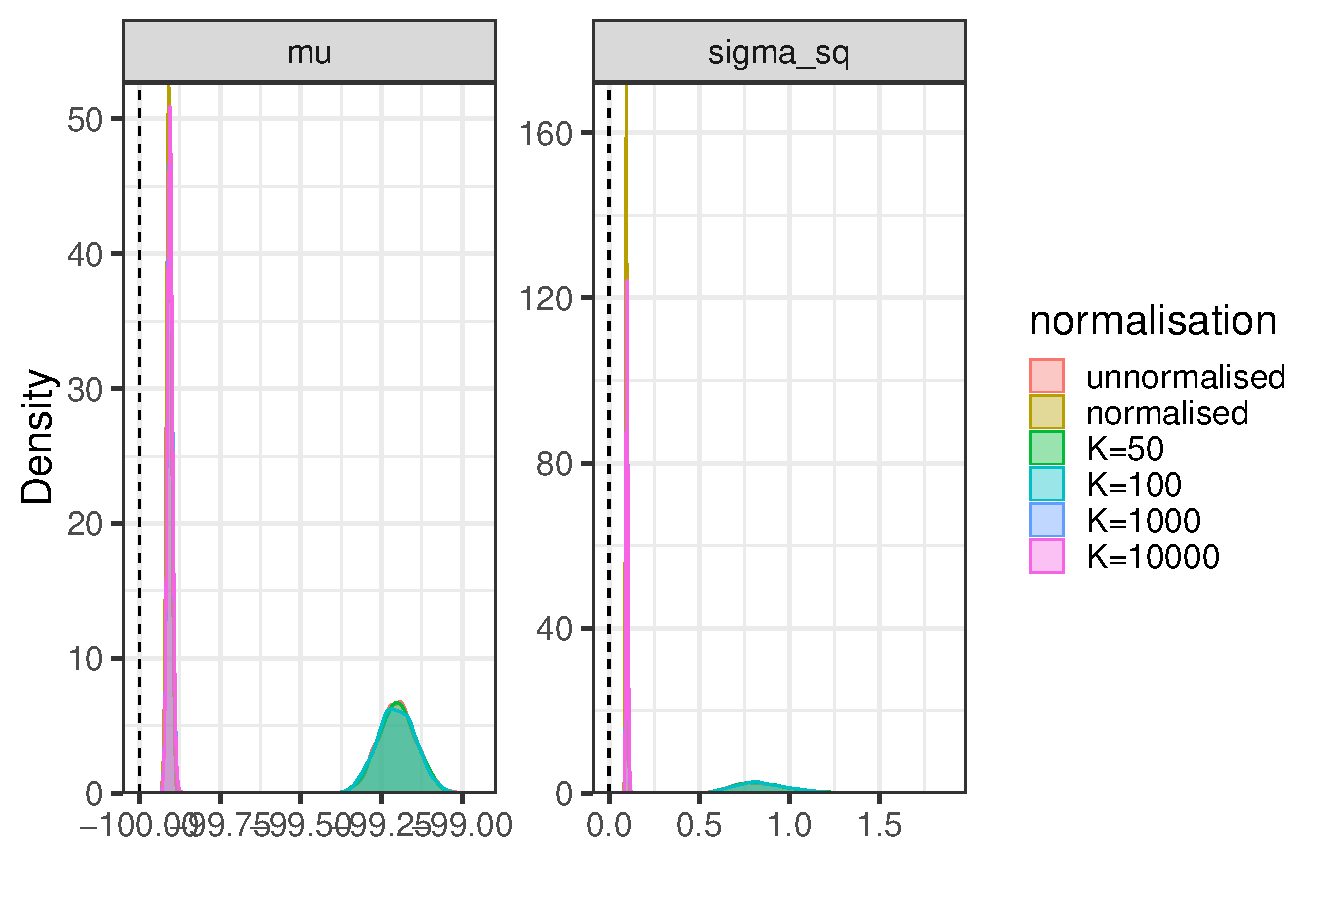
\includegraphics[width=7cm]{../figures/parameter_posterior_Gaussian.pdf}}
% \hfill
% \subfigure[Inverse-Gaussian]{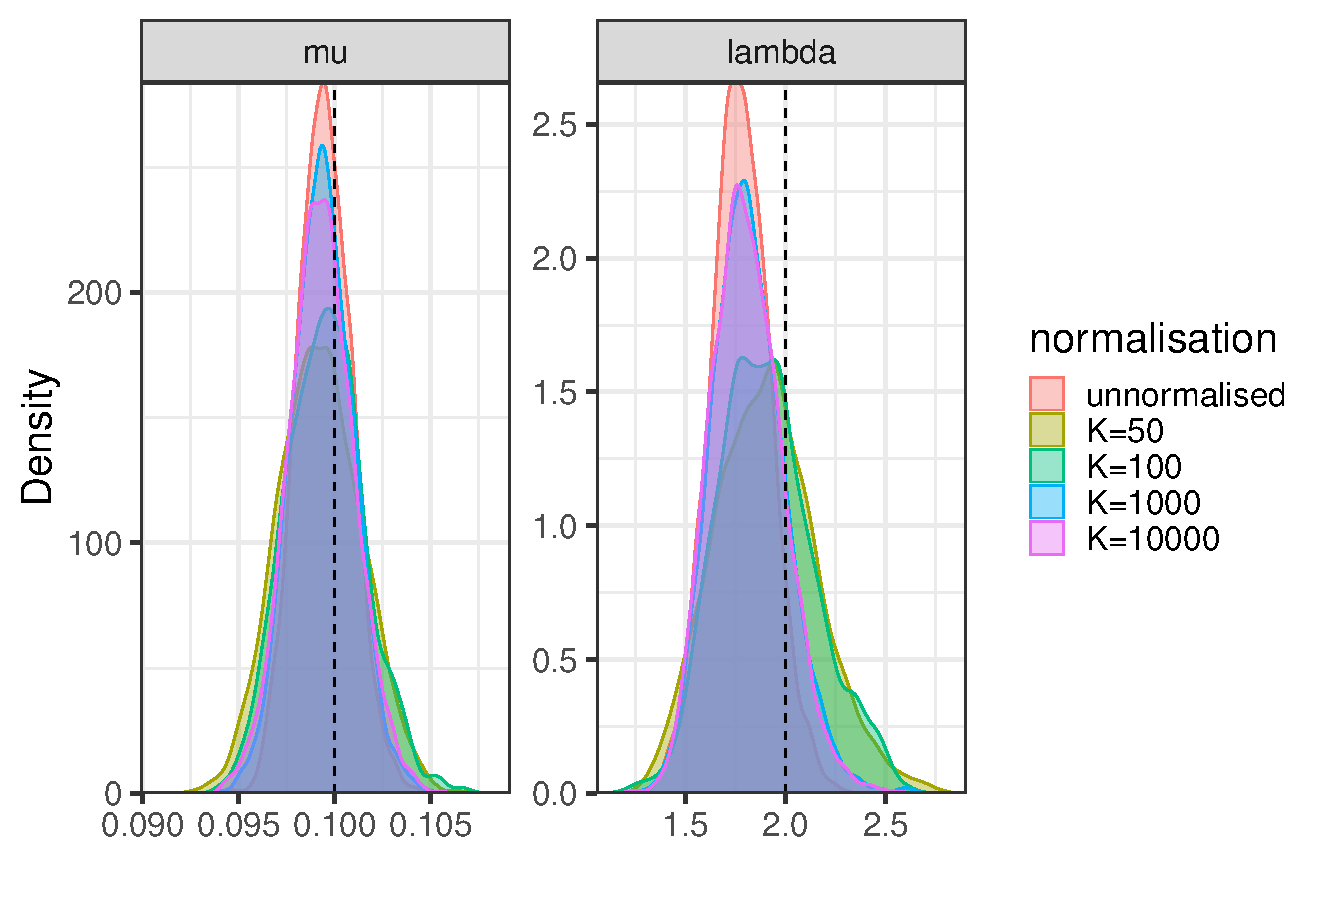
\includegraphics[width=7cm]{../figures/parameter_posterior_invgaussian.pdf}}\\
% \hfill
% \subfigure[Linear regression]{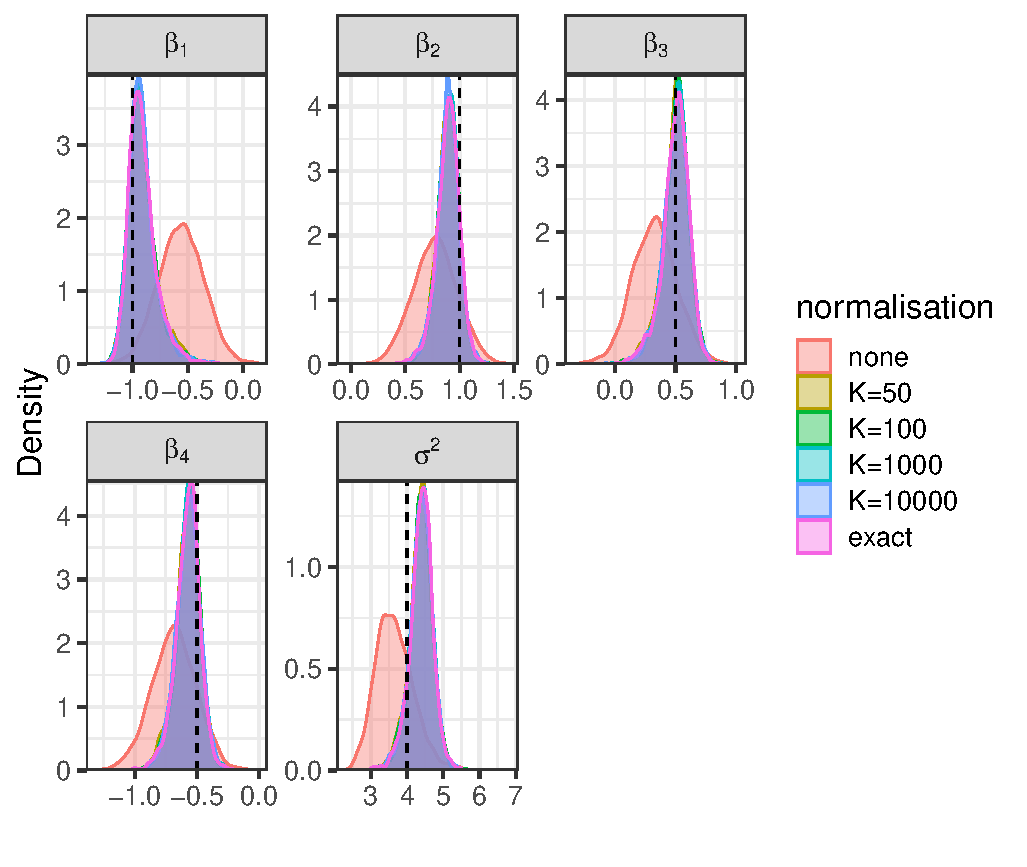
\includegraphics[width=7cm]{../figures/parameter_posterior_Regression.pdf}}
% \hfill
% \subfigure[Logistic regression]{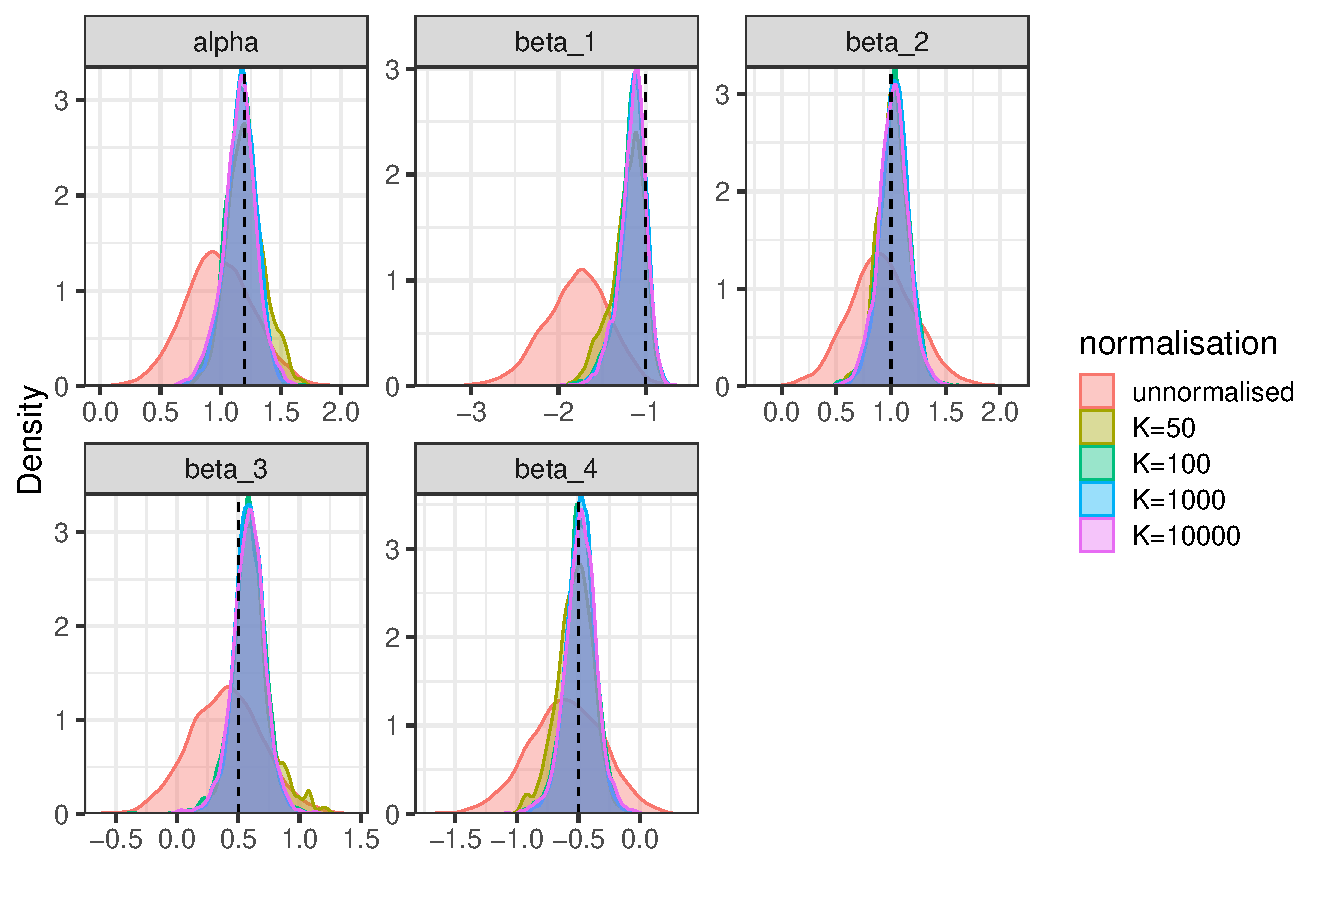
\includegraphics[width=7cm]{../figures/parameter_posterior_LogisticRegression.pdf}}
% \hfill
% \caption{\textbf{The posterior distribution of parameters of interest under normalised and unnormalised models}.
% The panels (and colours) correspond to the posterior distribution of the parameter $a_0$ when $c(a_0)$ is accounted for and when it is not included.
% Vertical lines mark the data-generating parameter values.
% }
% \label{fig:parameter_estimates}
% \end{figure}
\end{document}
